\documentclass[journal=jcisd8,manuscript=article,layout=two-column]{achemso}
\setkeys{acs}{articletitle=true,etalmode=truncate,maxauthors=20}
% compact text: 9 pt body
\renewcommand{\normalsize}{\fontsize{9}{11}\selectfont}
\renewcommand{\large}{\fontsize{11}{11}\selectfont}
\renewcommand{\Large}{\fontsize{12}{11}\selectfont}
\renewcommand{\LARGE}{\fontsize{15}{11}\selectfont}
\renewcommand{\small}{\fontsize{9}{10}\selectfont}
\renewcommand{\footnotesize}{\fontsize{7}{9}\selectfont}
\usepackage{enumitem}
\setstretch{1.125}
\setlength{\columnsep}{6.5mm}
\setlength\bibsep{1pt}
\usepackage[version=4]{mhchem}
\usepackage{calc}
\usepackage{booktabs}
\usepackage{caption}
\captionsetup{font=footnotesize,labelfont=bf}
\usepackage{graphicx}
\usepackage{multirow}
\usepackage{array,tabularx}
\usepackage{amsmath,amssymb}
\usepackage{siunitx}
\DeclareSIUnit{\angstrom}{\text{\AA}}
\sisetup{range-phrase=--, range-units=single}
\newcommand{\tcr}[1]{{\textcolor{red}{#1}}}
\newcommand{\tco}[1]{{\textcolor{orange}{#1}}}
\newcommand{\tcb}[1]{{\textcolor{black}{#1}}}
\usepackage{pifont}
\usepackage[english]{babel}
\IfFileExists{droidsans.sty}{\usepackage{droidsans}}{}
\usepackage{lmodern}
\usepackage{charter}
\usepackage[T1]{fontenc}
\usepackage[dvipsnames]{xcolor}
\usepackage[most]{tcolorbox}

\usepackage[compact]{titlesec}
\usepackage{xr}
\makeatletter
\newcommand*{\addFileDependency}[1]{\typeout{(#1)}\@addtofilelist{#1}\IfFileExists{#1}{}{\typeout{No file #1.}}}
\makeatother
\newcommand*{\myexternaldocument}[2][]{\externaldocument[#1]{#2}\addFileDependency{#2.tex}\addFileDependency{#2.aux}}
\usepackage[hidelinks]{hyperref}
\myexternaldocument[S-]{ESI_V3}
\AtBeginDocument{\renewcommand{\normalsize}{\fontsize{9}{11}\selectfont}}
\renewcommand{\dbltopfraction}{0.95}\renewcommand{\topfraction}{0.92}\renewcommand{\textfraction}{0.05}
\renewcommand{\floatpagefraction}{0.75}\renewcommand{\dblfloatpagefraction}{0.75}
\setlist{nosep,leftmargin=*}
\graphicspath{{MS_Figures_V3/}}
\newcommand{\ET}{E^{(2)}}
\newcommand{\BX}{BondX Studio}
\newcommand{\yes}{\ding{51}}
\newcommand{\no}{--}
\newcommand{\kcal}{kcal\,mol$^{-1}$}

\author{Soumyajit Karmakar\textsuperscript{a}$^{*}$}
\author{Sabyashachi Mishra\textsuperscript{a}}
\email{soumyajitkarmakar9991@kgpian.iitkgp.ac.in, mishra@chem.iitkgp.ac.in}
\affiliation{\textsuperscript{a}Department of Chemistry, Indian Institute of Technology Kharagpur, India, 721302}
\title[]{BondX Studio: Screening Geometric Halogen Contacts with Force-Field-Consistent QM Models, NBO Analysis, and ALMO-EDA}
\abbreviations{XB, NBO, ALMO-EDA, QM/MM}
\keywords{halogen bond, $\sigma$-hole, NBO, ALMO-EDA, QM/MM, force field, protonation, molecular dynamics, web tool}

\begin{document}
\sloppy

%% ---------------------------------------------------------------------
\begin{abstract}
% Short C--X$\cdots$Y contacts (X = Cl, Br, or I) in protein structures are routinely called halogen bonds on the basis of distance and angle alone, although crowding, a hydrogen bond to the halogen, or a poor Lewis base can produce the same geometry. Testing such an assignment by quantum chemistry requires a correctly protonated model of the binding site, consistent charges, and exact bookkeeping of every atom, which is why the test is rarely done. \BX{} is a free, single-file browser application that automates this chain: it detects contacts, follows them through molecular dynamics trajectories, builds QM cluster and QM/MM models with AMBER or CHARMM protonation states and charges, writes Gaussian~16 and Q-Chem inputs, and maps the NBO and ALMO-EDA outputs back onto the original atoms. Its NBO screen classes each contact as orbital-supported, inconclusive, or not supported, using a grey zone whose width is derived from the spread over methods and models, and it flags contacts in which a hydrogen bond to the halogen dominates. All outputs of 2200 generated inputs matched their manifests. On the HAL59 benchmark, the screen supported 53 of 56 halogen bonds, left three weak ones inconclusive, and supported none of the controls; however, it also supports bent contacts that are repulsive and compressed contacts that are losing binding, so the geometric limits remain part of every decision. Among 13 further contacts that pass the geometric test but involve poor Lewis bases, it supported two. Of nine distinct protein contacts, five were supported, three were inconclusive, and one was not supported. A re-analysis of published hIYD release simulations showed that 43 of 56 published NBO values were intramolecular donation and that none of 18 backbone-amide contacts remains supported once the amide is restored.

\tcb{Short C--X$\cdots$Y contacts (X = Cl, Br, or I) in biomolecular structures are often assigned as halogen bonds from geometry alone, although crowding, competing hydrogen bonds, and weak Lewis bases can produce similar arrangements. BondX Studio is a browser-based, single-file application that detects these contacts, follows them in trajectories, constructs force-field-based QM-cluster and electrostatically embedded QM/MM inputs, and maps NBO and ALMO-EDA results onto the original atoms. It does not run quantum-chemistry calculations. Its NBO screen reports valence donation into $\sigma^*$(C--X), competing donation from the halogen into nearby X--H antibonds, and an operational classification; these labels describe orbital donation, not binding. For the 29 HAL59 dimers with C-bound Cl, Br, or I donors, valence $\Sigma E^{(2)}$ correlates with CCSD(T)/CBS binding energies with Spearman $\rho$ = 0.73 (p = 8.0 $\times$ $10^{-6}$); 27 are labelled supported and two inconclusive, while 23 pass the present T1 acceptor and geometry scope. The three nominal controls all fail T1 and therefore do not test NBO specificity. Four rigid, T1-passing angle-scan structures have repulsive counterpoise energies but are NBO-supported, demonstrating that $\Sigma E^{(2)}$ alone does not establish attraction. Of nine distinct protein contacts, five are supported, three inconclusive, and one not supported. Re-analysis of 56 published hIYD outputs identifies 43 intramolecular contributions; additional intact-amide calculations show that backbone-N assignments depend on the model and level of theory. BondX Studio is therefore presented as a traceable screening workflow, not a binding-energy predictor.}


\end{abstract}

\paragraph*{Keywords} Halogen bond, $\sigma$-hole, NBO, ALMO-EDA, QM/MM, force-field charges, protonation, molecular dynamics, web application

%% =====================================================================
\section{Introduction}

A halogen atom X (Cl, Br, or I) bound to carbon carries an anisotropic charge distribution, because the region on the extension of the C--X bond is depleted of electron density and often positive. This $\sigma$-hole attracts lone pairs and $\pi$ systems, and the resulting directional contact, the halogen bond (XB), grows stronger from Cl to Br to I and prefers a nearly linear C--X$\cdots$Y arrangement.\cite{Clark2007,Desiraju2013,Cavallo2016,KolarHobza2016} Halogen bonds have been identified in proteins and nucleic acids, where backbone carbonyl O atoms are frequent partners,\cite{Auffinger2004,Voth2009,Scholfield2013,Sirimulla2013} and because heavier halogens can raise affinity in a predictable way while many approved drugs carry halogens,\cite{Lu2009,Wilcken2013,Hardegger2011,Smith2014,BenedettoTiz2022} the topic has become a routine part of structure-based design: PubMed lists between 222 and 290 halogen-bond records per year since 2017 (ESI Section~\ref{S-sec:counts}).\cite{PubMed2026}

Most of these studies assign XBs from distances and angles with fast and widely adopted interaction profilers.\cite{Salentin2015,Adasme2021,Jubb2017,Bouysset2021,Young2022} A short contact, however, is a hypothesis rather than a proof, since it may be enforced by a crowded pocket, the halogen may point sideways, the partner may be a poor Lewis base such as an amide nitrogen, or the halogen belt may accept a hydrogen bond from an N--H or O--H group. An electronic-structure test can discriminate between these cases, but it is laborious: a QM model must be cut from the structure, missing hydrogens need sensible protonation states, cut bonds need caps, the fragment charges must be right, and the environment needs a dielectric or point charges that are consistent with an established force field. The QM output must then be mapped back onto the original atoms, where a single wrong index changes the answer. In our earlier study of human iodotyrosine deiodinase (hIYD), we combined a geometric screen with NBO calculations by hand,\cite{Karmakar2026} and the re-analysis presented below shows how easily such a manual workflow goes wrong.

Here we present \BX{}, which performs the whole chain in a web browser without installation. Structure files are read locally, every step lists its assumptions, and every default is editable and logged; the program writes the QM inputs and reads the outputs but does not run quantum chemistry itself. We describe the method, test the atom bookkeeping and the NBO screen on benchmark dimers, protein complexes, and contacts with poor Lewis bases, quantify how much the QM/MM settings matter, and apply the workflow to published hIYD trajectories, distinguishing throughout what the software does correctly from what the chosen level of theory provides.

%% =====================================================================
%\section{Literature Survey and Standpoint}
\section{\tcb{Related Work}}
Table~\ref{tab:lit} summarizes the themes of the XB literature that shape the design of \BX{}. The IUPAC definition describes the XB as mainly electrostatic,\cite{Desiraju2013} whereas energy decomposition studies give a more varied picture: Thirman \emph{et al.} traced the binding trend of CX$_3$I donors to charge transfer,\cite{Thirman2018} and \v{R}ez\'a\v{c} and de la Lande estimated the charge-transfer (CT) share at about 10\% of the interaction energy.\cite{Rezac2017CT} Because this share depends on both the definition and the system, \BX{} reports the NBO donation, the NPA charge transfer, and the ALMO-EDA CT term side by side and treats none of them as an observable.

\begin{table*}[t]
\caption{Halogen-bond literature by theme and its use in \BX{}}
\label{tab:lit}
\footnotesize
\newcolumntype{L}[1]{>{\raggedright\arraybackslash}p{#1}}
\begin{tabularx}{\textwidth}{@{}L{2.4cm} L{4.6cm} >{\raggedright\arraybackslash}X L{3.9cm}@{}}
\toprule
Theme & Key reports & Main message & Use in \BX{} \\
\midrule
Definition, $\sigma$-hole & IUPAC,\cite{Desiraju2013} Clark,\cite{Clark2007} Cavallo\cite{Cavallo2016} & A positive cap on X; near-linear geometry & Angle window $140^\circ\le\theta_1\le180^\circ$ \\
Nature of the bond & Thirman,\cite{Thirman2018} \v{R}ez\'a\v{c} and de la Lande,\cite{Rezac2017CT} Kol\'a\v{r} and Hobza\cite{KolarHobza2016} & Electrostatics, dispersion, polarization, and CT all contribute, and their shares are debated & NBO screen beside ALMO-EDA and $\chi_\mathrm{CT}$ \\
Benchmarks & XB51,\cite{Kozuch2013} X40,\cite{Rezac2012X40} GMTKN55/HAL59\cite{Goerigk2017} & CCSD(T)/CBS binding energies of small dimers & Validation set (HAL59) \\
Biomolecules & Auffinger,\cite{Auffinger2004} Voth,\cite{Voth2009} Scholfield,\cite{Scholfield2013} Sirimulla\cite{Sirimulla2013} & XBs occur in proteins and DNA; C=O groups and rings are common partners & Acceptor classes and ring criterion \\
Drug design & Lu,\cite{Lu2009} Hardegger,\cite{Hardegger2011} Wilcken,\cite{Wilcken2013,Wilcken2012} Smith,\cite{Smith2014} Benedetto Tiz\cite{BenedettoTiz2022} & Heavier halogens bind more strongly, and many drugs carry Cl, Br, or I & Cut-offs for each halogen \\
Force fields & Jorgensen,\cite{Jorgensen2012} Ibrahim,\cite{Ibrahim2011} Scholfield (ffBXB),\cite{Scholfield2015} Ford and Ho\cite{FordHo2016} & Atom-centred charges miss the $\sigma$-hole; extra points or anisotropic terms add it & QM for the halogen, MM for the environment; extra points removed on reading \\
Detection tools & PLIP,\cite{Salentin2015,Adasme2021} Arpeggio,\cite{Jubb2017} ProLIF,\cite{Bouysset2021} BINANA\,2,\cite{Young2022} HBAT\,2,\cite{HBAT2} HalBS\cite{HalBS2025} & Fast, but geometric criteria only & Tier T1 \\
Density and orbital analysis & QTAIM,\cite{Bader1991} NCIPLOT,\cite{Johnson2010,ContrerasGarcia2011} Multiwfn,\cite{LuChen2012} NBO,\cite{Reed1988,Glendening2019} ALMO-EDA,\cite{Khaliullin2007,Horn2016} FMO-PIEDA\cite{Fedorov2007} & Bond paths, NCI surfaces, $n\to\sigma^*$ donation, and the CT/POL split characterize a contact, but each needs a QM model & Tiers T3b and T4 \\
QM-model and QM/MM set-up & RINRUS,\cite{Summers2021} QSite,\cite{Murphy2000QSite} ChemShell,\cite{Lu2019ChemShell} Senn and Thiel,\cite{SennThiel2009} Lin and Truhlar,\cite{LinTruhlar2005} Kulik\cite{Kulik2016} & QM-region selection, boundary charges, and model size change the results & Tier T3a: RC, RCD, and Z1--Z3 schemes; size tests \\
Scoring functions & XBScore,\cite{Zimmermann2015} VinaXB\cite{Koebel2016} & Empirical or QM-fitted XB terms for docking & Not used; BXQI only orders evidence \\
Our earlier study & Karmakar and Mishra\cite{Karmakar2026} & Geometry overcounts XBs in hIYD & The workflow; re-analysis in this work \\
\bottomrule
\end{tabularx}
\end{table*}

Interaction profilers such as PLIP, Arpeggio, ProLIF, BINANA, and HBAT detect XBs from distances and angles,\cite{Salentin2015,Adasme2021,Jubb2017,Bouysset2021,Young2022,HBAT2} HalBS uses XB geometry for structure validation,\cite{HalBS2025} and commercial suites such as Maestro, MOE, and Discovery Studio flag XBs in their interaction viewers.\cite{Maestro,MOE,DiscoveryStudio} These tools suit large surveys but give no electronic information. The established electronic tests, QTAIM bond paths and NCI surfaces,\cite{Bader1991,Johnson2010,ContrerasGarcia2011} are available in Multiwfn and NCIPLOT,\cite{LuChen2012,ContrerasGarcia2011} and NBO and ALMO-EDA are available in standard QM programs,\cite{Reed1988,Horn2016} yet all of them start from a wavefunction of a model that the user must build. RINRUS automates the selection, trimming, and capping of QM-cluster models from residue interaction networks,\cite{Summers2021} and QM/MM programs such as QSite (with Jaguar) and ChemShell set up and run embedded calculations,\cite{Murphy2000QSite,Bochevarov2013,Lu2019ChemShell} but none of these starts from a list of halogen contacts or returns a decision for each contact, and FMO-PIEDA, which gives pair interaction energies in whole proteins,\cite{Fedorov2007} suits detailed studies rather than screening. \BX{} therefore sits between the geometric profilers and the expert QM analyses and replaces neither: its geometric tier is comparable to the profilers, its QM tiers rely on standard programs, and its contribution is an automated, traceable, and force-field-consistent link between them. Table~\ref{tab:compare} compares the documented features.

\begin{table*}[t]
\caption{Features of existing tools and \BX{} (\yes{}: available; \no{}: not available; n.r.: not reported in the cited documentation)}
\label{tab:compare}
\footnotesize\setlength{\tabcolsep}{2.6pt}
\resizebox{\textwidth}{!}{%
\begin{tabular}{@{}lcccccccccccc@{}}
\toprule
Feature & PLIP & Arpeggio & ProLIF & BINANA\,2 & HalBS & XBScore, & Schr\"odinger & MOE, & Multiwfn, & RINRUS & ChemShell & \BX{} \\
 & & & & & & VinaXB & suite$^a$ & DS & NCIPLOT & & & \\
 & \cite{Adasme2021} & \cite{Jubb2017} & \cite{Bouysset2021} & \cite{Young2022} & \cite{HalBS2025} & \cite{Zimmermann2015,Koebel2016} & \cite{Maestro,Murphy2000QSite,Bochevarov2013} & \cite{MOE,DiscoveryStudio} & \cite{LuChen2012,ContrerasGarcia2011} & \cite{Summers2021} & \cite{Lu2019ChemShell} & this work \\
\midrule
XB detection by geometry & \yes & \yes & \yes & \yes & \yes & \yes & \yes & \yes & \no & \no & \no & \yes \\
Halogen--$\pi$ contacts & \no & \yes & n.r. & n.r. & n.r. & \no & n.r. & n.r. & \no & \no & \no & \yes \\
XB contacts along MD trajectories & \no & \no & \yes & \no & \no & \no & \no$^b$ & n.r. & \no & \no & \no & \yes \\
XB energy term or score & \no & \no & \no & \no & \no & \yes & n.r. & n.r. & \no & \no & \no & ranking only \\
QM-cluster or QM-region building & \no & \no & \no & \no & \no & \no & \yes & \no & \no & \yes & \no$^c$ & \yes \\
Force-field charges for QM/MM embedding & \no & \no & \no & \no & \no & \no & \yes & \no & \no & \no & \yes & \yes \\
Electronic analysis of a contact & \no & \no & \no & \no & \no & \no & \yes$^d$ & \no & \yes & \no & \no & \yes$^e$ \\
Energy decomposition & \no & \no & \no & \no & \no & \no & n.r. & \no & n.r. & \no & \no & \yes$^e$ \\
Runs the QM calculation itself & \no & \no & \no & \no & \no & \no & \yes & \no & \no & \no & \yes & \no \\
Decision per halogen contact & \no & \no & \no & \no & \no & \no & \no & \no & \no & \no & \no & \yes \\
Runs in a browser without a server & \no & \no & \no & \yes & \no & \no & \no & \no & \no & \no & \no & \yes \\
\bottomrule
\end{tabular}}

\footnotesize{$^a$Maestro with Jaguar, QSite, and Desmond. $^b$The Desmond simulation-interaction analysis reports hydrogen-bond, hydrophobic, ionic, and water-bridge contacts. $^c$QM/MM environment; the QM region is defined by the user. $^d$Jaguar computes wavefunction properties, including NBO, for a model that the user builds. $^e$Reads NBO (Gaussian~16, tested) and ALMO-EDA (Q-Chem, tested) outputs; the QM jobs are run by the user.}
\end{table*}

%% =====================================================================
\section{Method and Implementation}

Figure~\ref{fig:flow} shows the workflow, which is organized in tiers T0--T5 that carry the same labels in the program, the text, and the ESI. The user runs the QM jobs between tiers T3a and T3b, and every contact receives an NBO decision before the energy decomposition and the ranking.

\begin{figure*}[p]
\centering
\includegraphics[width=\textwidth,height=0.86\textheight,keepaspectratio]{Fig1_workflow.pdf}
\caption{Tiers of \BX{}. Each box lists what the tier does and, in its lower strip, the equation behind its score. Arrows show the flow of data; a single structure skips tier T2. The user runs the QM jobs between tiers T3a and T3b. The NBO screen sorts every contact into one of three classes, and all three classes are reported and ranked. ESI Section~\ref{S-sec:eq} defines every symbol, and ESI Table~\ref{S-tab:params} lists every parameter.}
\label{fig:flow}
\end{figure*}

\subsection{Architecture and privacy}
\BX{} is one HTML file of about \SI{0.5}{MB} that holds the force-field tables, the engine with all scientific code, and the interface. The engine is plain JavaScript, so the same code runs in Node.js for the automated tests, for batch work, and for the paper scripts, which call it through a command-line front end. Structure, trajectory, and QM output files are read by the browser and never leave the computer. The program makes three kinds of network request, which the footer of every page lists: downloads from RCSB when the user enters a PDB ID,\cite{Berman2000} the 3Dmol.js viewer library from its content delivery network,\cite{Rego2015} and, on the hosted site only, an anonymous page-view counter that receives the page address, the browser type, and the screen size but never a structure, a file, or a result; a copy of the file opened from disk never contacts the counter. The interface (Figure~\ref{fig:ui}) has one page per tier, pages for batch screening, crystal structures, parameters, and equations, and a tutorial whose last page lists the capabilities and the tested routes.

\begin{figure*}[t]
\centering
% Original composite screenshot replaced by separate supplied panel crops.
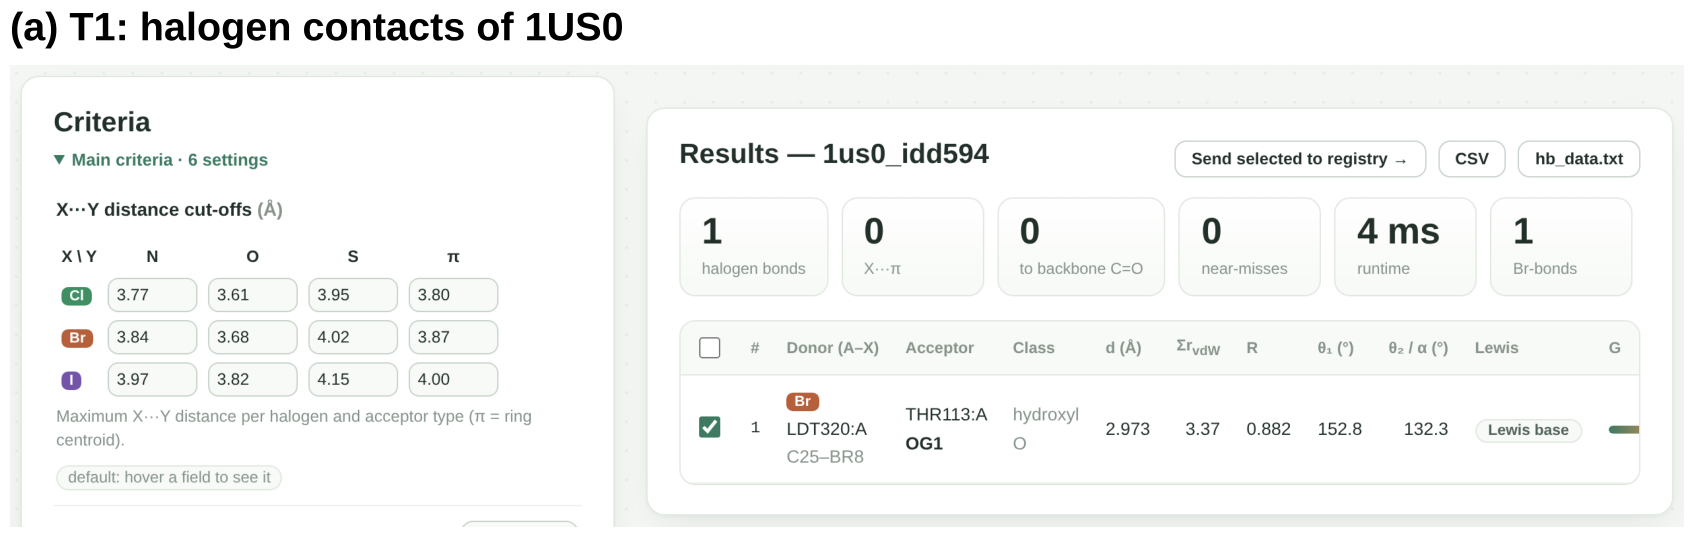
\includegraphics[width=0.86\textwidth]{Fig2a_T1_300dpi.png}\\[1mm]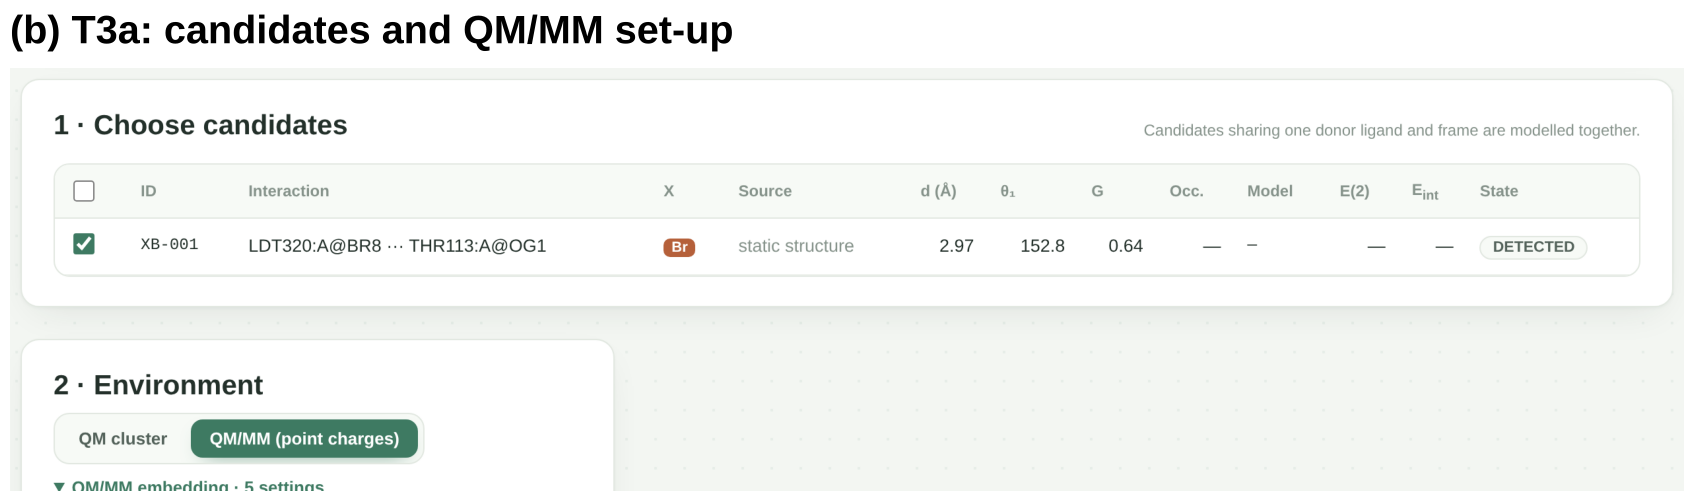
\includegraphics[width=0.86\textwidth]{Fig2b_T3a_300dpi.png}\\[1mm]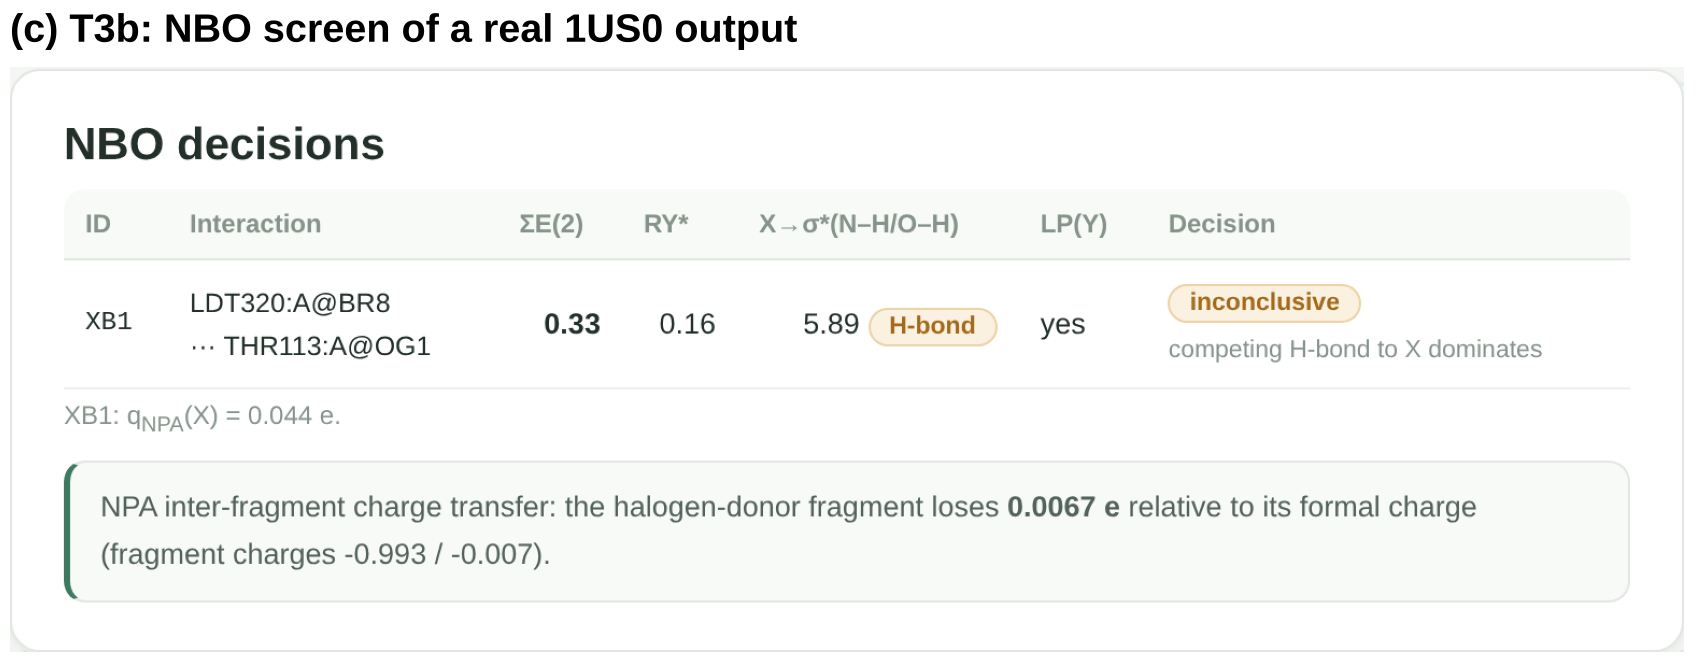
\includegraphics[width=0.86\textwidth]{Fig2c_T3b_300dpi.png}
% Original caption retained for reference.
% \caption{The \BX{} interface for 1US0 with the inhibitor IDD594. (a) Tier T1 with its distance cut-offs and the contact table. (b) Tier T3a with the candidate list and the choice between a cluster and a QM/MM model. (c) Tier T3b for the real NBO output of the default 1US0 cluster, with the valence decision value, the Rydberg part, the summed X$\to\sigma^*$(N--H/O--H) donation, and the decision, which carries the flag for a dominant competing hydrogen bond. Each page opens with its assumptions (not shown), and every setting shows its default. The 3D viewer loads 3Dmol.js from the internet and is therefore absent from these offline screenshots; ESI Figure~\ref{S-fig:screens} shows further pages.}}
\caption{\tcb{Separate, tightly cropped interface panels for the 1US0--IDD594 example. (a) T1 geometric detection and distance cut-offs. (b) T3a candidate selection and QM/MM setup. (c) T3b NBO analysis, including valence donation, Rydberg contribution, competing X$\to\sigma^*$(N--H/O--H) donation, and the decision flag. The three supplied screenshot panels are placed separately. The 3D viewer is absent from these offline screenshots; ESI Figure~\ref{S-fig:screens} shows further pages.}}
\label{fig:ui}
\end{figure*}

\subsection{Tier T0: structure input}
\BX{} reads PDB and PQR files and fetches entries from RCSB; a PQR file brings its own charges, so protonation states from PDB2PQR and PROPKA,\cite{Jurrus2018,Olsson2011} or from any other tool, can be used directly. Alternate locations follow the first conformer, bonds are assigned from covalent radii with a tolerance of \SI{0.45}{\angstrom}, residues are classed as protein, nucleic acid, water, ion, or ligand, and every input file receives a SHA-256 hash. Virtual sites, such as the $\sigma$-hole extra point (EP) of a halogen, lone-pair sites, and the M site of TIP4P water, carry a charge without a nucleus; \BX{} removes them on reading and maps DCD and XYZ frames that contain them onto the remaining atoms, because an EP would otherwise be counted as a hydrogen on the halogen.

\subsection{Tier T1: geometric detection}
\begin{figure*}[tbp]
\centering
\includegraphics[width=0.84\textwidth]{Fig3_T1_model.pdf}
\caption{Geometric model of tier T1. (a) Atom acceptor A--X$\cdots$Y--R, where A is the carbon bound to the halogen X, Y is the acceptor atom, and R is an atom bound to Y; the dashed spheres have the Bondi radii $r_\mathrm{X}$ and $r_\mathrm{Y}$, the blue cap marks the $\sigma$-hole, and the red belt marks the negative region of X. (b) Ring acceptor A--X$\cdots$Ct, where Ct is the ring centroid and $\alpha$ is the angle between the X$\cdots$Ct line and the ring normal $n$. (c) The three terms of the score and the score $G$, shown for the Br$\cdots$O cut-off, with the default cut-offs in the table (ESI Table~\ref{S-tab:cutoffs}); all values are editable.}
\label{fig:model}
\end{figure*}

% Original wording retained for reference; revised wording follows.
% Donors are C-bound Cl, Br, and I atoms of ligands and modified residues, with fluorine off by default. Acceptors are protein N, O, and S atoms, nucleic-acid N and O atoms, and the aromatic rings of Phe, Tyr, Trp, and the nucleobases, while His rings, water, and ligand or cofactor rings (for example, the isoalloxazine of a flavin) are optional. A candidate XB must satisfy two conditions: the distance $d$(X$\cdots$Y) must not exceed the pair cut-off, and the angle $\theta_1$ (A--X$\cdots$Y) must lie between \ang{140} and \ang{180}, with $\alpha \le \ang{60}$ in addition for a ring (Figure~\ref{fig:model}). The geometric score combines three terms,
\tcb{Tier T1 is defined for chlorine, bromine, and iodine atoms covalently bound to carbon in ligands or modified residues; fluorine donors are excluded by default. The supported acceptors are protein N, O, and S atoms, nucleic-acid N and O atoms, and aromatic rings of Phe, Tyr, Trp, and nucleobases; His rings, water, and ligand or cofactor rings remain optional. A candidate contact must satisfy its pair-specific distance cut-off and $140^\circ\leq\theta_1\leq180^\circ$; ring contacts additionally require $\alpha\leq60^\circ$ (Figure~\ref{fig:model}). HAL59 contains 56 nominal halogen-bond dimers, but 27 have non-C-bound donors (including F--I, Br--Br, F--Cl, F--Br, NBS, and NIS). These are retained as exploratory electronic-structure cases only and are excluded from T1 performance calculations. In particular, FI$\cdots$pyridine ($\Sigma E^{(2)}=72.2$~kcal~mol$^{-1}$) lies outside the implemented donor scope. The scope-matched C--X analysis therefore contains 29 dimers; 23 also have acceptors within the current T1 acceptor scope, while six P- or F-acceptor dimers have no default T1 acceptor cut-off. The geometric score combines distance, approach direction, and acceptor orientation as defined below.}

\begin{gather}
R=\frac{d}{r_\mathrm{X}+r_\mathrm{Y}},\qquad g_d=\mathrm{clip}\!\left(\frac{R_\mathrm{cut}-R}{R_\mathrm{cut}-0.85}\right)\\
g_\theta=\mathrm{clip}\!\left(\frac{\theta_1-140^\circ}{40^\circ}\right),\quad G=\left[g_d\,g_\theta\left(\tfrac12+\tfrac12 g_2\right)\right]^{1/3}
\end{gather}
% Original wording retained for reference; revised wording follows.
% where $r$ are Bondi radii,\cite{Bondi1964} a ring centroid has $r = \SI{1.77}{\angstrom}$, clip limits a value to the range 0--1, and $g_2$ rewards a $\theta_2$ (X$\cdots$Y--R) near \ang{120} or, for a ring, a small $\alpha$ ($g_2 = 1-\alpha/60^\circ$). The iodine cut-offs come from our earlier hIYD study,\cite{Karmakar2026} and the Br and Cl values follow from them by the difference in halogen radius (about 0.13~\AA{} from I to Br and 0.07~\AA{} from Br to Cl); rounded to 0.01~\AA{}, they lie at 1.09--1.14 times the Bondi sum for atom acceptors (ESI Table~\ref{S-tab:cutoffs}). Because $g_d$ is constant below $R = 0.85$, $G$ does not penalize compressed contacts, so \BX{} flags every contact with $R < 0.80$ as short and offers an optional linear penalty, which is off by default because the strongest benchmark XBs have $R \approx 0.69$ at equilibrium. Poor Lewis bases are kept with a flag and a reason, namely N atoms whose lone pair is delocalized (backbone amide N, Asn ND2, Gln NE2, and Trp NE1) and protonated N atoms (Lys NZ and the Arg guanidinium). The batch page applies T1 to many PDB entries, and the crystal page applies it to CIF and XYZ files with periodic images.
\tcb{The radii used for normalization are Bondi radii (Cl 1.75, Br 1.85, I 1.98, N 1.55, O 1.52, and S 1.80~\AA{}); an aromatic centroid uses 1.77~\AA{} (ESI Table~\ref{S-tab:cutoffs}). For atom acceptors, $g_2=\exp[-((\theta_2-\theta_{2,\mathrm{opt}})/40^\circ)^2]$, where the implemented optimum is $180^\circ$ for sp, $120^\circ$ for sp$^2$, and $109.5^\circ$ for sp$^3$ acceptors. The acceptor hybridization is inferred heuristically from local covalent connectivity and available heavy-atom geometry; when it cannot be assigned, the sp$^2$ reference is used. Ring acceptors retain $g_2=\mathrm{clip}(1-\alpha/60^\circ)$. The common Gaussian width is 40$^\circ$. Thus, a linear nitrile nitrogen (sp) is evaluated against a $180^\circ$ optimum; at $180^\circ$, its factor is $g_2=1$, rather than approximately 0.105 under the former fixed $120^\circ$ rule. The geometry output reports the inferred hybridization and selected $\theta_2$ target. The radii are Bondi radii, but the distance cut-offs are operational screening limits inherited from the earlier hIYD analysis and shifted empirically: I-to-Br shifts are 0.13--0.14~\AA{}, whereas the Br-to-Cl shift is 0.07~\AA{}. The Br--Cl Bondi-radius difference is 0.10~\AA{}, so this tabulated shift is not a direct radius subtraction. Likewise, the N--O cut-off separation is 0.15--0.16~\AA{}, larger than their 0.03~\AA{} Bondi-radius difference. The cut-offs are therefore not derived solely from van der Waals radii, and no radius-only recalibration is claimed. Because $g_d$ is constant below $R=0.85$, compressed contacts are not penalized by the default score; contacts with $R<0.80$ are flagged as short, and an optional linear penalty is available. Poor Lewis bases are retained with flags for delocalized lone pairs (backbone amide N, Asn ND2, Gln NE2, and Trp NE1) and protonated nitrogen atoms (Lys NZ and Arg guanidinium N). Hydrogens are not required for T1. The batch page applies T1 to multiple PDB entries, and the crystal page applies it to CIF and XYZ files with periodic images.}



\subsection{Tier T2: persistence in dynamics}
\BX{} reads DCD, multi-model PDB, and multi-frame XYZ trajectories and applies the T1 test to every frame, using the minimum-image convention for orthorhombic boxes. The occupancy is $f=N_\mathrm{on}/N_\mathrm{frames}$, the residence time $\tau$ is the mean length of unbroken runs converted to picoseconds with the spacing $\Delta t$ of the analysed frames, and the persistence score is
\begin{equation}
D=f\,\bigl[1-\exp(-\tau/\tau_0)\bigr]^{p}
\end{equation}
% Original wording retained for reference; revised wording follows.
% with $\tau_0=\SI{100}{ps}$ and $p=\tfrac14$. The exponent applies only to the residence factor, which then saturates quickly, so that a contact surviving for a few $\tau_0$ is scored almost by its occupancy, whereas a contact that flickers for single frames is penalized. Because a run cannot be shorter than $\Delta t$, the residence factor is at least 0.89 when $\Delta t = \tau_0$ and approaches 1 for coarser sampling; \BX{} then states that $D$ is practically equal to $f$ and that residence times are resolved only to one frame spacing. Contacts below a reporting threshold (10\% occupancy by default, adjustable down to zero) are hidden but kept, and the representative frame of a contact, which has the shortest $d$ and, among equal distances, the largest $\theta_1$, goes to tier T3a. Frames from biased simulations such as umbrella-sampling windows are counted without reweighting, so their occupancies describe each window rather than the unbiased ensemble, for which WHAM or MBAR weights would be needed.\cite{Kumar1992,ShirtsChodera2008}
\tcb{with $\tau_0=\SI{100}{ps}$ and $p=\tfrac14$. The residence factor saturates rapidly: when the saved-frame interval approaches or exceeds $\tau_0$, $D$ is practically equal to the occupancy $f$, and the residence time is resolved only to the saved-frame spacing. Contacts below a reporting threshold (10\% occupancy by default, adjustable down to zero) are hidden but retained, and the representative frame (shortest $d$, with the largest $\theta_1$ breaking ties) is sent to T3a. Frames from biased simulations, including umbrella windows, are counted without reweighting; the resulting occupancies are window-specific and are not unbiased ensemble populations. WHAM or MBAR reweighting would be required for unbiased occupancies, and neither a finely sampled trajectory validation nor such reweighting is reported here.}

\subsection{Tier T3a: force-field-consistent QM models}
\paragraph{Force-field data and protonation.}
Residue templates and atomic charges were extracted from the OpenMM force-field files.\cite{Eastman2017} The tables hold AMBER ff14SB\cite{Maier2015} and ff19SB\cite{Tian2020} with the OL15 DNA\cite{GalindoMurillo2016} and OL3 RNA\cite{Zgarbova2011} parameters, CHARMM36\cite{Best2012} with the patches for termini and protonation variants applied during extraction, the water models TIP3P,\cite{Jorgensen1983} SPC/E,\cite{Berendsen1987} and OPC3,\cite{IzadiOnufriev2016} and the Joung--Cheatham,\cite{Joung2008} Li--Merz,\cite{LiMerz2015} and CHARMM ion charges. The default states correspond to pH~7 (Asp and Glu anionic, Lys and Arg cationic, Cys and Tyr neutral, and His as HIE), and residue names or hydrogens in the file override them. Because a fixed His default is a weak choice for QM/MM work, \BX{} lists every His within \SI{8}{\angstrom} of a halogen with a warning and recommends a pKa tool such as PROPKA, whose result can be loaded as a PQR file.\cite{Olsson2011}

\paragraph{Ligands.}
Without a MOL2 file, ligand hydrogens and the ligand charge come from one Kekul\'e structure in which each sp$^2$ carbon receives one double bond, the keto form is preferred, an sp$^2$ ring N without a double bond carries one H, and a pyridinium-type N with three neighbours carries $+1$; acid groups (carboxylic, phosphoric, phosphonic, sulfonic, and sulfuric) are deprotonated. Aliphatic amines, tetrazoles, and acyl sulfonamides are usually charged at pH~7 but cannot be assigned safely from connectivity alone, so \BX{} flags them, offers to protonate basic amines, and recommends a MOL2 file with a state from Epik, PROPKA, or a similar tool.\cite{Shelley2007,Olsson2011} The PDB formula (FORMUL record) provides an independent check of the hydrogen count, and ligand hydrogens present in the file are kept when they fit the structure.

\paragraph{The QM region.}
% Original wording retained for reference; revised wording follows.
% Fragment~1 is the whole halogenated ligand, and fragment~2 contains the whole acceptor residues together with two kinds of neighbours that the chemistry requires: when the acceptor is a backbone atom, the neighbouring residue is added, so that a backbone N keeps the C=O group of the preceding residue and remains an amide rather than becoming an amine with a link hydrogen; and every residue with an N--H or O--H group within \SI{3.6}{\angstrom} of the halogen, water included, is added, so that a competing hydrogen bond to the halogen lies inside the QM region. An optional shell of whole residues within a chosen distance of X can be added on top, and cut bonds receive link hydrogens. Added O--H and S--H hydrogens of Ser, Thr, Tyr, and Cys are rotated to the rotamer with the best hydrogen bond, where N, O, and C-bound halogen acceptors are scored alike, so that the rule neither favours nor excludes an O--H$\cdots$X hydrogen bond. When a halogen-directed rotamer and another rotamer fit about equally well, \BX{} reports the tie and lets the user force either rotamer, so that both models can be built and their decisions compared; hydrogens from a PQR file, for example from PDB2PQR or Reduce,\cite{Jurrus2018,Word1999Reduce} are used as given. Fragment charges come from the template formal charges and the ligand structure, and \BX{} warns about an odd electron count, about an anionic fragment written with a basis set that lacks diffuse functions, and about an incomplete ligand.
\tcb{Fragment~1 is the whole halogenated ligand, and fragment~2 contains the whole acceptor residues together with the neighbouring residues needed to preserve backbone chemistry and competing N--H/O--H contacts. When the acceptor is a backbone atom, the preceding residue is included so that a backbone N retains its carbonyl partner and remains an amide rather than being converted into an amine by a link hydrogen. Residues carrying an N--H or O--H group within 3.6~\AA{} of the halogen, including water, are also included. An optional shell of whole residues can be added, and cut bonds receive link hydrogens. Added Ser, Thr, Tyr, and Cys hydroxyl hydrogens are oriented using the implemented hydrogen-bond ranking; near-ties are reported so that alternative rotamers can be examined. The ligand charge and fragment charges derive from the selected structure/force-field templates or supplied MOL2/PQR data. Anionic models require diffuse functions for reliable energies. The protein NBO calculations reported here for 1US0 ($-1$), 2W0S ($-2$), and 4GQL ($-3$) used def2-TZVP without diffuse functions despite the software warning. Gaussian does not provide def2-TZVPD as a built-in basis keyword, but the basis can be supplied explicitly using Gen/GenECP. No completed def2-TZVPD NBO sensitivity calculations for these three protein models are available; the 2W0S counterpoise comparison is not an NBO diffuse-basis test.}


\paragraph{Environment, input files, and manifest.}
% Original wording retained for reference; revised wording follows.
% A cluster model can sit in a PCM dielectric, by default $\varepsilon=4$,\cite{BaroneCossi1998,Cossi2003,Tomasi2005} whereas a QM/MM model uses electrostatic embedding with MM point charges from a PQR file, a MOL2 file, or the chosen force field. By default, all residues of the structure enter; MM residues within \SI{6}{\angstrom} of a halogen carry explicit hydrogens with their template charges, which keeps the N--H and O--H dipoles closest to the $\sigma$-hole, and farther away each hydrogen charge is added to its heavy atom, which keeps every residue charge exact. The boundary atom M1 is the MM atom bonded to the QM region, and its charge is moved to the M1--M2 bond midpoints (RC, the default) or, in the RCD scheme recommended by Lin and Truhlar, also restores the M2--M1 bond dipoles;\cite{LinTruhlar2005} the Z1, Z2, and Z3 schemes, which delete the charges of the M1, M1--M2, or M1--M3 atoms, are also available. The MM region is not neutralized and has no solvent, \BX{} reports its net charge, and QM--MM van der Waals terms, which do not affect the NBO analysis of a single point, are not included. The program writes NBO single-point inputs for Gaussian~16 with molecule reorientation switched off,\cite{g16} and a manifest records every QM atom with its PDB origin, the fragment charges, the force field, all parameters, and all assumptions. Inputs for NBO in ORCA, which requires the licensed NBO~7 program, and in Q-Chem are written only after the user unlocks untested routes.\cite{Neese2022,Glendening2019,Epifanovsky2021}
\tcb{A cluster model can sit in a PCM dielectric, by default $\varepsilon=4$, whereas a QM/MM model uses electrostatic embedding with MM point charges from a PQR file, MOL2 file, or selected force field. By default, all residues enter the MM region; residues within 6~\AA{} of X retain explicit hydrogens with template charges, while farther hydrogen charges are folded onto their parent heavy atoms. The boundary atom M1 is treated with RC by default; RCD and Z1--Z3 alternatives are available. The embedding is electrostatic, non-polarizable, and contains no explicit solvent; QM--MM van der Waals terms are not included in the single-point NBO analysis. The MM region is not neutralized and its net charge is reported. A spatially uniform additive constant in the electrostatic potential does not change the electronic density, but a net MM charge distributed over the environment does not generate a spatially uniform potential: it produces a position-dependent electric field and field gradients at the QM region. The available field correlations (six contacts, $\rho=-0.14$; 54 pooled model variants, $\rho=0.17$) do not establish insensitivity of $\Sigma E^{(2)}$ to the MM field. No counterion, charge-neutralization, or charge-scaling sensitivity calculations have been completed, so the embedded NBO results remain model-dependent. The tested NBO input route is Gaussian~16 with NBO~3.1. ORCA NBO and Q-Chem NBO routes are not validated; ORCA is used for counterpoise energies and Q-Chem for ALMO-EDA.}

\subsection{Tier T3b: the NBO screen}
\BX{} reads the second-order perturbation table of the NBO output\cite{Reed1988,NBO31} after comparing the output geometry with the manifest, and an atom-count, element, or coordinate mismatch blocks the screen. The decision value is the valence donation into the $\sigma$-hole,
\begin{equation}
\Sigma\ET=\sum\ET\!\left[n_\mathrm{Y}\!\rightarrow\!\sigma^*_\mathrm{A-X}\right],
\end{equation}
% Original wording retained for reference; revised wording follows.
% where $n_\mathrm{Y}$ is a lone pair of the T1 acceptor atom Y, so that lone pairs of other atoms and donation within the halogenated molecule never count; a ring acceptor uses the $\pi\to\sigma^*_\mathrm{A-X}$ terms of its ring bonds, and when NBO describes a strongly polarized A--X bond as two ions, the donation into the vacant lone pair LP$^*_\mathrm{X}$ takes the place of $\sigma^*_\mathrm{A-X}$. Donation into Rydberg orbitals of the halogen is reported beside the decision value but not counted, because it depends strongly on the basis set. $\Sigma\ET$ is a second-order estimate for one localization scheme and one level of theory rather than an observable or a binding energy, and we use it only as a screen: each contact is orbital-supported ($\Sigma\ET \ge 0.8$~\kcal{}), inconclusive ($0.3 \le \Sigma\ET < 0.8$~\kcal{}), or not supported ($\Sigma\ET < 0.3$~\kcal{}). The centre of this grey zone, 0.5~\kcal{}, is a convention equal to the default print threshold of NBO for couplings within one unit (between units, such as a ligand and a protein residue, NBO prints couplings down to 0.05~\kcal{}), whereas the width of the zone was derived from the spread of $\Sigma\ET$ over levels of theory and model variants (see Results). Three flags qualify a decision without changing its class. The first marks a dominant competing hydrogen bond, which applies when the halogen lone pairs donate more into N--H or O--H antibonds of fragment~2 than the acceptor donates into $\sigma^*_\mathrm{A-X}$ (and at least 0.5~\kcal{}); such a contact ranks after the unflagged supported contacts. The second marks ring acceptors, which in HAL59 give about a quarter of the $\Sigma\ET$ per unit binding energy of N acceptors, and the third keeps the poor-Lewis-base flag of tier T1, because NBO can place a lone pair on such an acceptor in its Lewis structure. \BX{} also reports whether NBO prints a lone pair on Y and the NPA charge transfer between the fragments, which in a protein cluster sums every ligand--environment contact and is therefore not specific to one XB.
\tcb{where $n_\mathrm{Y}$ is a lone pair of the T1 acceptor atom Y, so that donation from other atoms and intramolecular donation within the halogenated ligand are excluded. Ring acceptors use the $\pi\to\sigma^*_{\mathrm{A-X}}$ terms of the ring bonds; for strongly polarized A--X bonds represented ionically by NBO, donation into the vacant halogen LP$^*$ orbital is used where appropriate. Rydberg donation is reported separately and is not included in the decision value. $\Sigma E^{(2)}$ is a second-order orbital-donation estimate for one localization scheme and level of theory, not an observable or binding energy. The operational labels are supported ($\Sigma E^{(2)}\geq0.8$~kcal~mol$^{-1}$), inconclusive ($0.3\leq\Sigma E^{(2)}<0.8$~kcal~mol$^{-1}$), and not supported ($\Sigma E^{(2)}<0.3$~kcal~mol$^{-1}$). The selected 0.5~kcal~mol$^{-1}$ reference value lies within the inconclusive interval; it is a convention, not a calibrated threshold or the arithmetic midpoint (0.55~kcal~mol$^{-1}$). NBO prints inter-unit couplings down to 0.05~kcal~mol$^{-1}$, while the 0.50~kcal~mol$^{-1}$ print threshold applies to couplings within one unit. The width of the 0.3--0.8 interval was selected from the spread across levels of theory and model variants; an independent binding-energy calibration and class-specific thresholds have not been performed. In the 29 C-bound-donor HAL59 subset, median valence $\Sigma E^{(2)}_{\mathrm{core}}/E_{\mathrm{bind}}$ ratios are N (n=12), 1.61; O (n=5), 1.09; S (n=2), 1.56; ring (n=4), 0.46; P (n=4), 2.01; and F (n=2), 0.95. P and F lie outside the current T1 acceptor scope, and the O median is approximately 33\% lower than the N median. Three interpretive flags qualify the class without replacing it: (i) competing hydrogen bond, when halogen donation into an N--H/O--H antibond on the acceptor side dominates the scored donation; (ii) ring acceptor, for aromatic $\pi$ acceptors; and (iii) poor Lewis base, for amide and selected side-chain nitrogens whose lone pairs may be weak or delocalized. These flags do not independently establish binding. The reported NPA charge transfer in a protein cluster sums all ligand--environment contacts and is not specific to the individual halogen bond.}



\subsection{Tiers T4 and T5: ALMO-EDA and ranking}
\BX{} writes Q-Chem EDA2 inputs,\cite{Horn2016,Epifanovsky2021} by default at the $\omega$B97X-V/def2-TZVPD level with a counterpoise-corrected CT term and optionally with the COVP analysis, which isolates the dominant donor--acceptor orbital pairs of the CT term.\cite{Khaliullin2008COVP} It reads the frozen (FRZ), polarization (POL), and CT terms in \kcal{}, with $\Delta E_\mathrm{int}=E_\mathrm{FRZ}+E_\mathrm{POL}+E_\mathrm{CT}$, and reports the CT character $\chi_\mathrm{CT}=E_\mathrm{CT}/(E_\mathrm{POL}+E_\mathrm{CT})$, where $\chi_\mathrm{CT}\ge0.6$ marks a CT-driven and $\chi_\mathrm{CT}\le0.4$ a polarization-driven contact. Because fragment~2 holds every acceptor residue, the EDA terms of a protein cluster describe every contact between the ligand and fragment~2 rather than the XB alone.

For the ranking, each tier that can be evaluated gives a score between 0 and 1, namely $s_G = G$, $s_D = D$, $s_E = 1-\exp(-\Sigma\ET/E_0)$, and $s_C = 1-\exp[-\max(0,-\Delta E_\mathrm{int})/C_0]$ with $E_0 = 2$~\kcal{} and $C_0 = 2.4$~\kcal{}, so that a repulsive interaction gives $s_C = 0$. The BondX quality index is the weighted geometric mean of the available scores,
\begin{equation}
\mathrm{BXQI}=100\prod_{k\in\mathcal{A}} s_k^{\,w_k/\sum_{j\in\mathcal{A}} w_j},
\end{equation}
where $\mathcal{A}$ contains only the tiers that could be evaluated and the default weights are 0.25 ($G$), 0.2 ($D$), 0.3 ($E$), and 0.25 ($C$). A tier that cannot be evaluated, such as $G$ for an acceptor without a default cut-off, is left out rather than set to zero, and the EDA term can be switched off when fragment~2 holds more than the acceptor. Candidates are ordered first by the NBO decision (supported, supported with a dominant competing hydrogen bond, inconclusive, not supported, and not run) and then by BXQI, which has no grades and serves as an ordering convenience rather than a binding energy; a provenance code (for example, G$\cdot$D$\cdot$E$\cdot$C) lists the tiers behind each value.

\subsection{Assumptions, parameters, and provenance}
% Original wording retained for reference; revised wording follows.
% \BX{} has 97 adjustable parameters (ESI Table~\ref{S-tab:params}). Each tier page shows its parameters with their defaults, highlights changed values, offers a reset, and lists its assumptions in plain words (ESI Section~\ref{S-sec:assume}), which update after every change; parameter sets can be exported and imported, and an audit trail records every load, change, and result in the HTML report and the JSON run record.
\tcb{BondX Studio exposes 99 adjustable parameters (ESI Table~\ref{S-tab:params}), but they are not 99 independent decision thresholds. The parameters that directly control T1/NBO classification are the donor and acceptor scope, pair-specific distance cut-offs, the $\theta_1$ acceptance limit, the hybridization-dependent $\theta_2$ optimum and Gaussian width, the short-contact handling, the poor-Lewis-base and competing-hydrogen-bond flags, and the NBO supported/inconclusive boundaries. Other parameters govern file parsing, QM-region construction, force-field and embedding choices, output writing, or display. Each tier page shows defaults, highlights changed values, provides reset/export/import functions, and records settings and results in the HTML report and JSON run record.}


%% =====================================================================
\section{Computational Details}

\paragraph{Benchmark dimers and scans.}
% Original wording retained for reference; revised wording follows.
% HAL59 is part of GMTKN55\cite{Goerigk2017} and contains 45 XB51 dimers\cite{Kozuch2013} and 14 X40 dimers,\cite{Rezac2012X40} each with a CCSD(T)/CBS binding energy that we checked against the GMTKN55 files. Three dimers serve as controls (two fluoroarene--benzene stacks and FI$\cdots$FCCH, in which the iodine points away from the partner); because these are easy negatives, harder ones are treated separately below. Rigid scans of 12 dimers move the acceptor along the X$\cdots$Y line from 0.90 to 1.50 times its equilibrium distance $d_\mathrm{eq}$ (8 points), and rigid angle scans of six dimers rotate the acceptor about X so that $\theta_1$ runs from \ang{180} to \ang{120} (7 points) at fixed $d$ and $\theta_2$; because the partner is not relaxed, the bent geometries include steric repulsion that a relaxed contact would partly avoid.
\tcb{HAL59 is part of GMTKN55 and contains 45 XB51 dimers and 14 X40 dimers, each with a CCSD(T)/CBS binding energy checked against the GMTKN55 files. The benchmark includes 29 dimers with C-bound Cl, Br, or I donors, which define the primary donor-scope subset, and 27 additional dimers with non-C-bound donors, which are retained only as exploratory quantum-chemical examples. Six of the 29 C-bound cases have P or F acceptors outside the current T1 acceptor scope. The three nominal negative controls (two fluoroarene--benzene stacks and FI$\cdots$FCCH, where iodine points away) fail T1 and therefore test geometric exclusion rather than NBO specificity. Rigid distance scans of 12 dimers and rigid angle scans of six dimers were generated; because the acceptor was not relaxed, bent scan geometries may contain steric repulsion and do not replace relaxed, independently constructed hard-negative contacts.}

\paragraph{Protein test set.}
The PLIP project distributes 55 PDB files with literature-validated interactions,\cite{Adasme2021} of which four tests assert halogen bonds and three have Cl, Br, or I donors: 2W0S (Asn65),\cite{Caillat2008} 1P5E (Ile10 and Leu83),\cite{DeMoliner2003} and 4AGL (Leu145);\cite{Wilcken2012} the fourth, 3SHY (Tyr612),\cite{Xu2011} has a fluorine-only ligand. We added aldose reductase 1US0 with IDD594\cite{Howard2004} from the PDB2PQR test data, a file that lacks the NADP$^+$ cofactor, and built QM models for six systems: 1US0, 2W0S, 1P5E, 4AGL, 4GQL,\cite{Czarny2013} and 4DST.\cite{Maurer2012}

\paragraph{QM protocol.}
The NBO jobs used $\omega$B97X-D\cite{ChaiHeadGordon2008}/def2-TZVP\cite{WeigendAhlrichs2005} in Gaussian~16 (Revision B.01) with its built-in NBO~3.1,\cite{g16,NBO31} and all programs used the def2 effective core potential for iodine.\cite{Peterson2003} The ALMO-EDA jobs used $\omega$B97X-V\cite{Mardirossian2014,Vydrov2010}/def2-TZVPD\cite{Rappoport2010} in Q-Chem~6.2.2.\cite{Epifanovsky2021} Because Gaussian and ORCA have no ALMO-EDA, each EDA job has two partner jobs that give the counterpoise-corrected\cite{BoysBernardi1970} interaction energy, one in Gaussian ($\omega$B97X-D/def2-TZVP) and one in ORCA~5.0.1\cite{Neese2020,Neese2022} ($\omega$B97X-V/def2-TZVPD, RIJCOSX with the def2/J auxiliary basis\cite{Neese2009,Weigend2006}); the protein ORCA jobs also removed near-linearly dependent basis functions (overlap threshold $10^{-6}$) and used the DefGrid3 grid. The PCM cluster models used CPCM with $\varepsilon=4$,\cite{BaroneCossi1998,Cossi2003} and the EDA and counterpoise jobs of the protein clusters are gas-phase calculations. Table~\ref{tab:sets} lists all job sets. The level set D covers M06-2X,\cite{ZhaoTruhlar2008} B3LYP-D3(BJ),\cite{Becke1993,LYP1988,Grimme2010,Grimme2011} PBE0-D3(BJ),\cite{AdamoBarone1999,Grimme2010,Grimme2011} $\omega$B97X-D, and Hartree--Fock with def2-TZVP and three further basis sets with $\omega$B97X-D, and the protein variants test the force field, the boundary scheme, the embedding radius, the QM-region size, the environment (gas, PCM, or MM), and the His110 tautomer of 1US0.

% Original wording retained for reference; revised wording follows.
\tcb{The 89 protein models in set F used the following saved model choices: backbone-N sites at model boundaries were capped with link hydrogens when the preceding carbonyl was not included (including 4DST Gly75); added hydroxyl hydrogens retained their template rotamer (including the 1US0 Thr113 model); MM hydrogen charges were folded onto parent heavy atoms throughout the MM region; and the embedding radius was 15~\AA{}. The deposited 1US0 entry does not contain hydrogen coordinates for Thr113. Set G contains 17 hIYD challenge calculations, including 12 T1-passing poor-Lewis-base contacts and five Lewis-base comparison contacts. Among the 12 poor-Lewis-base cases, seven were not supported, three were inconclusive, and two were supported (Arg164 and Thr178). Set J contains three 4DST Gly75 calculations with the intact amide; all three gave zero valence donation and were not supported. Set K contains 18 hIYD backbone-N poses rebuilt with acetyl caps at the published level; 17 jobs terminated normally and one stopped while writing the NBO file after its complete NBO table had printed. Set K has no atom-by-atom manifest, so its outputs were checked against the saved geometries and must not be described as manifest-verified. These are saved model choices for one BondX Studio application; no application-edition distinction is made. The alternative 1US0 hydroxyl rotamer and a whole-structure QM/MM NBO calculation retaining explicit MM hydrogens have not been completed.}


\begin{table}[t]
\caption{QM input files written by \BX{} for this work}
\label{tab:sets}
\footnotesize\setlength{\tabcolsep}{2.2pt}
\begin{tabular}{@{}lp{2.75cm}rrrr@{}}
\toprule
Set & Content & NBO$^a$ & EDA$^b$ & CP$^c$ & Used$^d$ \\
\midrule
A & 59 HAL59 dimers & 177 & 59 & 236 & N, E, C \\
B & 12 dimers $\times$ 8 distances & 288 & 96 & 384 & N, E, C \\
C & 6 dimers $\times$ 7 angles & 126 & 42 & 168 & N, E, C \\
D & 12 dimers $\times$ 8 levels & 276 & -- & -- & N \\
E & 12 dimers $\times$ 3 EDA settings & -- & 36 & -- & E \\
F & 89 protein models & 267 & 9 & 36 & N, E$^e$, C$^f$ \\
G & 17 hIYD frames$^g$ & 17 & -- & -- & N \\
J & 4DST, intact amide$^g$ & 3 & -- & -- & N \\
K & 18 hIYD poses, acetyl cap & 18 & -- & -- & N \\
\midrule
 & Total: 2238 files & 1172 & 242 & 824 & \\
\bottomrule
\end{tabular}

% Original wording retained for reference; revised wording follows.
% \footnotesize{$^a$Inputs for Gaussian~16, ORCA, and Q-Chem in sets A--F (only the Gaussian jobs were used; Gaussian lacks def2-TZVPD, so set D has 84 Gaussian jobs) and Gaussian inputs in sets G--K. $^b$Q-Chem ALMO-EDA. $^c$Counterpoise interaction energy: one Gaussian job and three ORCA single points for each EDA job. $^d$N: Gaussian NBO; E: Q-Chem ALMO-EDA; C: Gaussian and ORCA counterpoise jobs. $^e$Six of nine EDA jobs finished. $^f$Gaussian: nine clusters; ORCA: eight clusters. $^g$Built with the defaults of \BX{}. Set K edits the published inputs by script. Two further sets in the repository (H, a level test of the marginal protein contacts, and I, 1US0 with NADP$^+$) gave no results and are not used.}
\tcb{\footnotesize{$^a$Inputs for Gaussian~16, ORCA, and Q-Chem were generated for sets A--F; Gaussian NBO jobs were the tested NBO calculations. Gaussian can use externally supplied def2-TZVPD through Gen/GenECP even though it has no built-in def2-TZVPD keyword. Sets G--K contain Gaussian NBO inputs. $^b$Q-Chem ALMO-EDA. $^c$Counterpoise interaction energy: one Gaussian job and three ORCA single points for each EDA job. $^d$N: Gaussian NBO; E: Q-Chem ALMO-EDA; C: Gaussian and ORCA counterpoise jobs. $^e$Six of nine EDA jobs finished. $^f$Gaussian: nine clusters; ORCA: eight clusters. $^g$The model-specific saved settings are described in the text. Set K edits the published inputs by script. Sets H (marginal-contact level test) and I (1US0 with NADP$^+$) produced no results and are not used.}}
\end{table}
\tcb{The 2,238 generated inputs comprise 1,172 NBO inputs, 242 Q-Chem ALMO-EDA inputs, and 824 counterpoise inputs. In the 2,200-input A--F status table, 370 Gaussian NBO jobs completed, 239/242 Q-Chem ALMO-EDA jobs completed, 206/206 Gaussian counterpoise jobs completed, and 615/618 ORCA counterpoise jobs completed. The 382 ORCA NBO inputs were not run, and 382 Q-Chem NBO outputs lacked the required second-order perturbation table. Sets G and J add 20 normally completed Gaussian NBO jobs, 17 of which (G) plus three (J) completed with saved-geometry checks, bringing the normally completed and manifest-checked Gaussian NBO outputs to 390. Set K adds 18 NBO outputs with no manifest: 17 terminated normally, and one stopped during output writing after the NBO table was produced. Generated inputs, completed jobs, and manifest-verified outputs are therefore distinct counts.}


\paragraph{hIYD release data.}
The hIYD data come from our earlier study:\cite{Karmakar2026} the hIYD dimer with reduced flavin (FMNhq) and the 3-iodotyrosine (I-Tyr) phenolate, simulated with AMBER ff14SB, GAFF,\cite{Wang2004GAFF} and TIP3P water and with an EP on the iodine. Umbrella sampling followed three release pathways, A, B, and C, each with 36 windows along the progress coordinate $\xi$ (3.8--\SI{8.8}{\angstrom} in steps of \SI{0.2}{\angstrom} and 9.8--\SI{18.8}{\angstrom} in steps of \SI{1}{\angstrom}), and each window ran for 25~ns with one frame every 20~ps. A cpptraj\cite{RoeCheatham2013} script kept every 5th to 12th frame and all residues within \SI{15}{\angstrom} of I-Tyr and removed water and ions, which leaves 11\,361 frames in 108 windows with 100--240~ps between the saved frames. We also read the 56 published QM-cluster outputs, computed with B3LYP-D3/6-311++G(d,p) and LANL2DZdp on iodine\cite{Check2001} in CPCM ($\varepsilon=4$) with NBO~3.1 in Gaussian~16.

\paragraph{Software tests and scripts.}
% Original wording retained for reference; revised wording follows.
% The engine has 120 automated tests, and a Playwright test drives the browser through every page, including the batch and crystal pages. Numbered scripts and the command-line front end produced every number, figure, and table (ESI Table~\ref{S-tab:scripts}), and the analysis steps were run three times in fresh folders with identical results apart from the timings. Spearman coefficients are given with 95\% bootstrap confidence intervals (10\,000 resamples), and timings used Node.js~22 on one core of a \SI{2.3}{GHz} Intel Xeon processor.
\tcb{The engine has 123 automated tests, including regression tests for the C-bound Cl/Br/I donor scope and the hybridization-dependent $\theta_2$ targets; the independent force-field reference comparisons pass. A Playwright test drives the browser through every page, including the batch and crystal pages. Numbered scripts and the command-line front end produced the paper analyses, figures, and tables (ESI Table~\ref{S-tab:scripts}). The revised T1 benchmark and figure-generation scripts were rerun after the donor-scope and hybridization changes. Spearman coefficients are reported with 95\% bootstrap confidence intervals where calculated; the reported correlations below are the direct values from the regenerated benchmark subset.}

%% =====================================================================
\section{Results and Discussion}

\subsection{Atom bookkeeping and force-field data}
% Original wording retained for reference; revised wording follows.
% All 2238 input files were generated without manual editing, and every Gaussian NBO job and every ORCA single point that terminated normally (all jobs of sets A--G and J, and 17 of 18 set-K jobs) returned an output whose atom order, elements, and coordinates matched the manifest and whose electron count matched the real atoms and the charge; set K, which edits published inputs, has no manifest and was checked by its geometry. Every residue template has an integer net charge in all three force fields, while the 5$'$ and 3$'$ nucleic-acid termini carry fractional charges that sum to $-1$ for each pair. Against the PDB2PQR reference files,\cite{Jurrus2018} the ff14SB charges agree exactly for all 5855 heavy atoms and, without folding, for all 5807 hydrogens of four proteins (ESI Table~\ref{S-tab:ffref}). Because both programs read the same AMBER parameter files, this comparison tests the template matching, the termini, and the protonation handling rather than the charges themselves; PDB2PQR ships CHARMM22 charges, which differ from the CHARMM36 tables only for tryptophan, so the CHARMM comparison is a consistency check and not a validation of CHARMM36.
\tcb{All 2,238 input files were generated without manual editing, but generation must not be conflated with execution or manifest validation. For sets A--F, 370 Gaussian NBO outputs completed and passed atom-by-atom manifest geometry checks; 382 ORCA NBO inputs were not run, and 382 Q-Chem NBO outputs did not contain the required second-order perturbation table. In sets G and J, 20 Gaussian NBO outputs completed and were checked against their saved geometries, giving 390 normally completed Gaussian NBO outputs with manifest geometry verification in the tested routes. Set K has no manifest: 17 of 18 jobs terminated normally and one stopped during NBO-file writing after its NBO table had printed; its values were compared with saved geometries, not manifests. Q-Chem ALMO-EDA completed for 239/242 jobs, Gaussian counterpoise for 206/206, and ORCA counterpoise for 615/618. The repository therefore supports the input-generation and completed-output counts stated above, not a claim that every generated input was run or every output matched a manifest. Every residue template has an integer net charge in the three force fields, while the 5-prime and 3-prime nucleic-acid termini carry fractional charges that sum to $-1$ for each pair. Against PDB2PQR reference files, the ff14SB charges agree exactly for all 5,855 heavy atoms and, without folding, all 5,807 hydrogens of four proteins (ESI Table~\ref{S-tab:ffref}). Because both programs read the same AMBER parameter files, this comparison tests template matching, termini, and protonation handling rather than independently validating the charge parameters themselves; the CHARMM comparison is a consistency check, not an independent validation of CHARMM36.}

\subsection{Geometric tier}
% Original wording retained for reference; revised wording follows.
% All 41 HAL59 dimers with N, O, S, or ring acceptors pass T1, the 15 dimers with P or F acceptors have no default cut-off, and all three controls fail (Figure~\ref{fig:t1}a). The geometric score correlates only moderately with the binding energy (Spearman $\rho = 0.71$ [0.51, 0.84], $n = 41$) and cannot separate a weak XB from a strong one at similar geometry; the three FI dimers with N acceptors, for example, have $G \ge 0.82$, although their binding energies range from 9.3 to 20.3~\kcal{}. Along the rigid scans, $G$ reaches zero at 1.10--1.35~$d_\mathrm{eq}$ for ten dimers, whereas the two strongest dimers (FI$\cdots$pyridine and H$_3$N$\cdots$BrF), which have very short equilibrium distances, keep $G>0$ up to 1.50~$d_\mathrm{eq}$ (ESI Figure~\ref{S-fig:scans}).
\tcb{The regenerated HAL59 analysis contains 29 dimers with C-bound Cl, Br, or I donors. Of these, 23 have N, O, S, or aromatic-ring acceptors within the present T1 scope; the remaining six C-bound-donor dimers have P or F acceptors without a default T1 cut-off. The 27 non-C-bound-donor dimers are excluded from T1 performance statistics. For the 23 scope-matched dimers, the geometric score has a Spearman correlation of $\rho=0.486$ ($p=0.0188$, $n=23$) with the CCSD(T)/CBS binding energy (Figure~\ref{fig:t1}a). This is a moderate association and does not establish binding or rank interaction strength reliably. The regenerated scores use the acceptor-hybridization-dependent $\theta_2$ target described above. Along the rigid distance scans, $G$ reaches zero at 1.10--1.35~$d_\mathrm{eq}$ for ten dimers, whereas two short-equilibrium-distance dimers retain nonzero scores to 1.50~$d_\mathrm{eq}$ (ESI Figure~\ref{S-fig:scans}).}

\begin{figure*}[t]
\centering
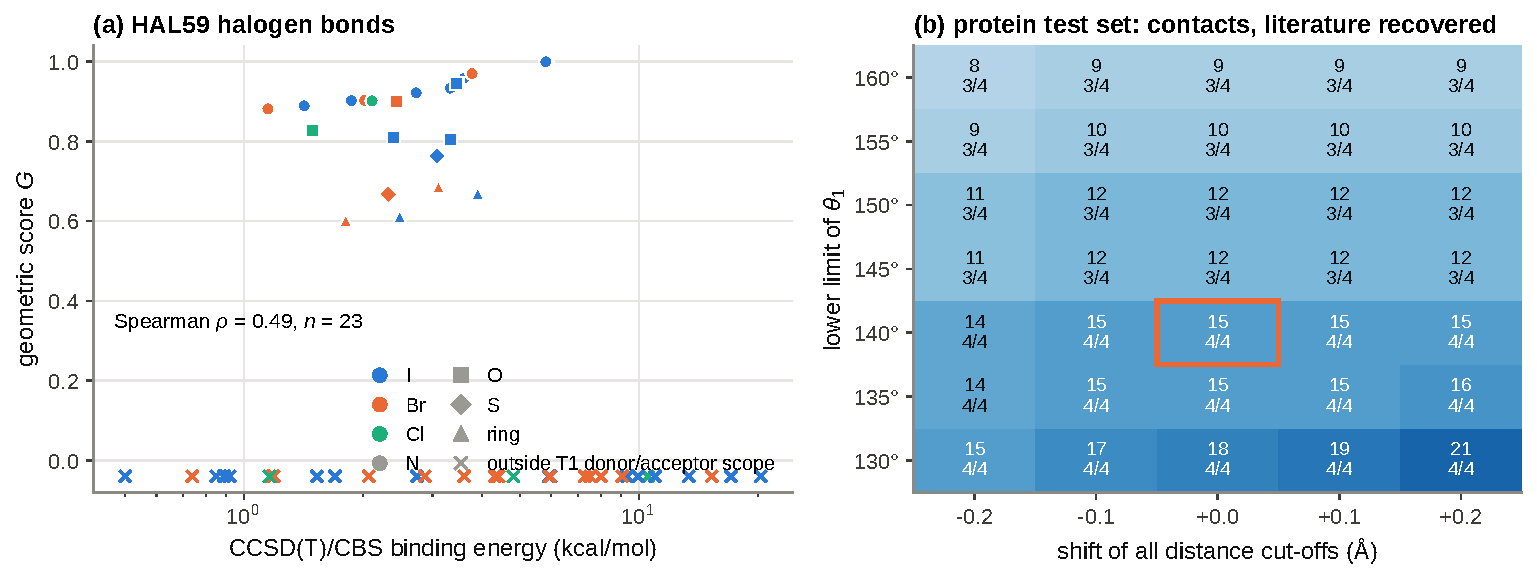
\includegraphics[width=0.92\textwidth]{Fig4_T1_benchmark.pdf}
% Original wording retained for reference; revised wording follows.
% \caption{Tier T1. (a) Geometric score $G$ against the CCSD(T)/CBS binding energy for the HAL59 halogen bonds (colour: halogen; shape: acceptor; crosses: P and F acceptors, which have no default cut-off); the bracket gives the 95\% bootstrap interval. (b) Contacts found in the protein test set (upper number, including chain replicas) and literature contacts recovered (lower number, out of four) for 35 parameter settings; the orange box marks the defaults.}
\caption{\tcb{Tier T1. (a) Geometric score $G$ against the CCSD(T)/CBS binding energy for the 23 HAL59 dimers with C-bound Cl, Br, or I donors and acceptors inside the current T1 scope. The six additional C-bound-donor dimers with P or F acceptors are outside the current T1 acceptor scope and are not included in this geometric correlation. (b) Contacts found in the protein test set (upper number, including chain replicas) and selected literature-annotated C--X contacts identified (lower number, out of four) for 35 parameter settings; the orange box marks the defaults.}}
\label{fig:t1}
\end{figure*}

% Original wording retained for reference; revised wording follows.
% On the protein test set, T1 analysed each of the 56 files in \SIrange{15}{325}{ms} and found 15 contacts in seven files (six entries and a polar-hydrogen copy of 4DST), which comprise nine distinct contacts, five replicas in other chains, and the 4DST contact counted again in its copy (ESI Table~\ref{S-tab:protT1}). \BX{} recovered all four literature contacts with Cl, Br, or I donors, namely Br$\cdots$OD1 Asn65 in 2W0S (\SI{2.69}{\angstrom}), Br$\cdots$O Leu83 and Br$\cdots$O Ile10 in 1P5E (2.90 and \SI{3.24}{\angstrom}; the latter weak by geometry, with $\theta_1 = \ang{144.1}$ and $G = 0.38$), and I$\cdots$O Leu145 in 4AGL (\SI{3.01}{\angstrom}). It also found Br12$\cdots$O Glu81 and Br13$\cdots\pi$ Phe80 in 1P5E, Br$\cdots$OG1 Thr113 in 1US0 (\SI{2.97}{\angstrom}), Cl$\cdots$O Pro232 in 4GQL, and Cl2$\cdots$N Gly75 in 4DST ($G = 0.12$, $\theta_2 = \ang{73}$), whose backbone amide N is flagged as a poor Lewis base. The fluorine-only ligand of 3SHY places its F atom \SI{3.85}{\angstrom} from Tyr612 OH, beyond every F cut-off, and with fluorine switched on, one of five F contacts in other files (F$\cdots$NE2 Gln483 at \SI{2.48}{\angstrom} in 6NHB) is most likely an N--H$\cdots$F hydrogen bond, which supports the default exclusion of fluorine. The angle limit controls detection more than the distance limit (Figure~\ref{fig:t1}b): a lower angle limit of \ang{130} finds up to 21 contacts and a limit of \ang{145} loses the Ile10 contact, whereas shifts of all distance cut-offs by $\pm\SI{0.2}{\angstrom}$ change the count by at most one.
\tcb{On the protein test set, T1 analysed each of the 56 files in 15--325~ms and found 15 contacts in seven files, comprising nine distinct contacts and chain replicas (ESI Table~\ref{S-tab:protT1}). Four selected literature-annotated contacts in these structures have C-bound Cl, Br, or I donors: Br$\cdots$OD1 Asn65 in 2W0S, Br$\cdots$O Leu83 and Br$\cdots$O Ile10 in 1P5E, and I$\cdots$O Leu145 in 4AGL. The NBO results support three of these four; Ile10 remains inconclusive ($\Sigma E^{(2)}=0.31$--$0.36$~kcal~mol$^{-1}$). This small selected set is descriptive and does not estimate general sensitivity across protein halogen bonds. Other detected contacts include Br12$\cdots$O Glu81 and Br13$\cdots\pi$ Phe80 in 1P5E, Br$\cdots$OG1 Thr113 in 1US0, Cl$\cdots$O Pro232 in 4GQL, and Cl2$\cdots$N Gly75 in 4DST; the latter is flagged as a poor-Lewis-base backbone amide. The fluorine-only ligand of 3SHY is outside the implemented donor scope. The angle limit controls detection more than the distance limit (Figure~\ref{fig:t1}b): relaxing the lower angular limit increases geometric candidates, whereas a limit of 145$^\circ$ loses Ile10; shifts of all distance cut-offs by $\pm0.2$~\AA{} change the count by at most one.}


\subsection{QM models and the MM field}
The default protein models contain 36--100 atoms (ESI Table~\ref{S-tab:models}), and their ligand charges are $-1$ for the IDD594 carboxylate (1US0), $-2$ for brivudine monophosphate (2W0S), and $-3$ for the phosphinic inhibitor of 4GQL, whereas the 1P5E inhibitor TBS is neutral with one triazole N--H; all models have an even electron count. The PDB formula confirms the ligand hydrogens wherever a FORMUL record exists, \BX{} rebuilt two polar ligand hydrogens missing from 4GQL, and it reported that the 4AGL ligand P84 has only 13 of its 21 heavy atoms, so the resolved part was completed with hydrogens from its Kekul\'e structure and its ranking refers to this truncated ligand. Over the whole test set, the ligand hydrogen count matches the formula for 191 of 214 complete ligand residues without metal, every mismatch is flagged, and in a polar-hydrogen-only copy of 4DST the program caught a missing indole N--H through an odd electron count.

% Original wording retained for reference; revised wording follows.
% The MM charges alone give the field component $E_{AX}$ along the A$\to$X axis at the halogen, where a positive value should deepen the $\sigma$-hole (Figure~\ref{fig:field}, ESI Table~\ref{S-tab:field}). Explicit hydrogens for MM residues within \SI{6}{\angstrom} of X shift $E_{AX}$ by $-0.14$ to $+0.18$~V\,\AA$^{-1}$ (unrounded differences) relative to folded hydrogen charges, which shows that folding near the halogen biases the field, whereas the RCD scheme changes $E_{AX}$ by at most 0.04~V\,\AA$^{-1}$ relative to RC, and CHARMM36 and ff14SB agree within 0.05~V\,\AA$^{-1}$ once explicit hydrogens are used (CHARMM36 writes fewer point charges, for example 914 instead of 1224 for 2W0S at \SI{15}{\angstrom}, because many of its aliphatic CH$_n$ groups are neutral and their folded heavy atoms carry no charge). The embedding radius matters more: \SI{15}{\angstrom} differs from the whole structure by up to 0.12~V\,\AA$^{-1}$, \SI{25}{\angstrom} by up to 0.08, and \SI{40}{\angstrom} by at most 0.01~V\,\AA$^{-1}$, so the default embeds the whole structure at negligible cost. The MM net charge is far from zero in several systems ($+5$~e for 2W0S and $+6$~e for 1P5E at \SI{15}{\angstrom}, and $-12$~e for the whole 2W0S structure), which makes a gas-phase QM/MM model a crude representation of the environment, although a uniform shift of the potential does not change the QM density.
\tcb{The MM charges alone give the field component $E_{AX}$ along the A$\to$X axis at the halogen (Figure~\ref{fig:field}, ESI Table~\ref{S-tab:field}). Explicit hydrogens for MM residues within 6~\AA{} of X shift $E_{AX}$ by $-0.14$ to $+0.18$~V~\AA$^{-1}$ relative to folded hydrogen charges, showing that folding near the halogen changes the local field. RCD changes $E_{AX}$ by at most 0.04~V~\AA$^{-1}$ relative to RC, while CHARMM36 and ff14SB agree within 0.05~V~\AA$^{-1}$ when explicit hydrogens are used. The embedding radius also matters: 15~\AA{} differs from the whole structure by up to 0.12~V~\AA$^{-1}$, 25~\AA{} by up to 0.08, and 40~\AA{} by at most 0.01~V~\AA$^{-1}$. The MM net charge is far from zero in several systems (+5~e for 2W0S and +6~e for 1P5E at 15~\AA{}, and $-12$~e for the whole 2W0S structure). Although a spatially constant potential shift would not alter the density, a spatially distributed net MM charge generates a nonuniform potential, electric field, and field gradients at the QM region. The within-contact field correlations (five contacts, $\rho=0.66$--0.97; 4DST remains near zero) and across-contact correlations ($\rho=-0.14$, $n=6$; pooled $\rho=0.17$, $n=54$) do not establish insensitivity of $\Sigma E^{(2)}$ to the net MM field. No controlled neutralization, counterion, or charge-scaling sensitivity calculations have been completed.}


\begin{figure*}[t]
\centering
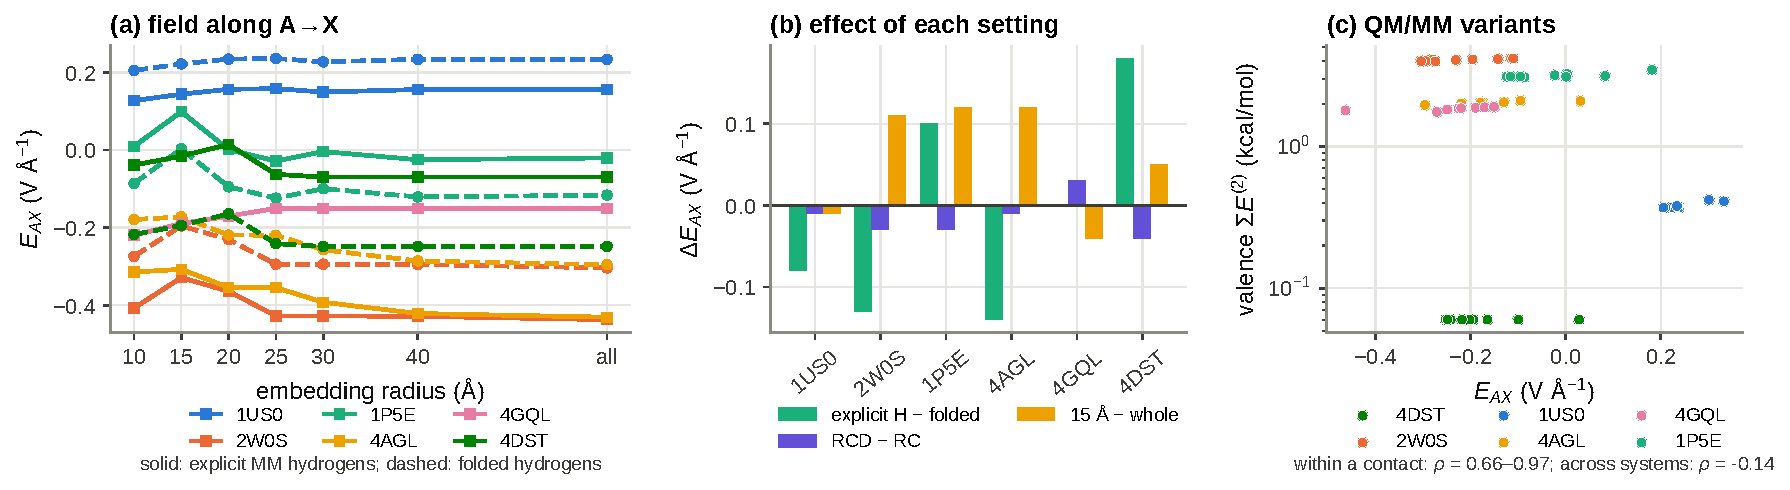
\includegraphics[width=\textwidth]{Fig5_embedding_field.pdf}
\caption{Field at the halogen from the MM point charges and its relation to $\Sigma\ET$. (a) $E_{AX}$ along the A$\to$X bond against the embedding radius (ff14SB, RC), with explicit MM hydrogens within \SI{6}{\angstrom} of X (solid) or folded hydrogen charges (dashed). (b) Change of $E_{AX}$ by explicit hydrogens, by the RCD boundary, and by truncation at \SI{15}{\angstrom}. (c) Valence $\Sigma\ET$ against $E_{AX}$ for the QM/MM variants of six contacts; the trend is clear within a contact but absent across systems.}
\label{fig:field}
\end{figure*}

Within one contact, $\Sigma\ET$ follows $E_{AX}$ over the QM/MM variants (Spearman $\rho = 0.66$--0.97 for five contacts with $n = 9$ each, while the sixth, 4DST, stays at $\Sigma\ET \le 0.07$), but across contacts the change of $\Sigma\ET$ from the cluster to the QM/MM model does not track $E_{AX}$ ($\rho = -0.14$, $n = 6$; pooled over all variants, $\rho = 0.17$, $n = 54$; Figure~\ref{fig:field}c and ESI Table~\ref{S-tab:m12}). The field is therefore useful for comparing settings for one contact, but it cannot replace the QM job or predict whether embedding strengthens a given XB.

\subsection{Energies at the default level}
The counterpoise energies characterize the default level of the energy tiers rather than \BX{} itself. The ORCA values reproduce the CCSD(T)/CBS binding energies of the 59 dimers with a mean absolute error of 0.40~\kcal{}, a root-mean-square error of 0.54~\kcal{}, and a mean signed error of $-0.07$~\kcal{} (Figure~\ref{fig:cp}a, ESI Table~\ref{S-tab:cphal}), as expected for $\omega$B97X-V/def2-TZVPD on HAL59,\cite{Goerigk2017} with the largest error for FI$\cdots$NH$_3$ (overbound by 1.62~\kcal{}). The ALMO-EDA totals agree with them within 0.05~\kcal{} (mean absolute error against CCSD(T)/CBS 0.39~\kcal{}), which is expected by construction at the same functional and basis and thus confirms that both programs received consistent geometries, charges, and fragments rather than providing an independent physical validation. $\chi_\mathrm{CT}$ ranges from 0.48 to 0.81, and the frozen term is repulsive in 23 of the 56 XBs, which are then held together by polarization and charge transfer.

\begin{figure*}[t]
\centering
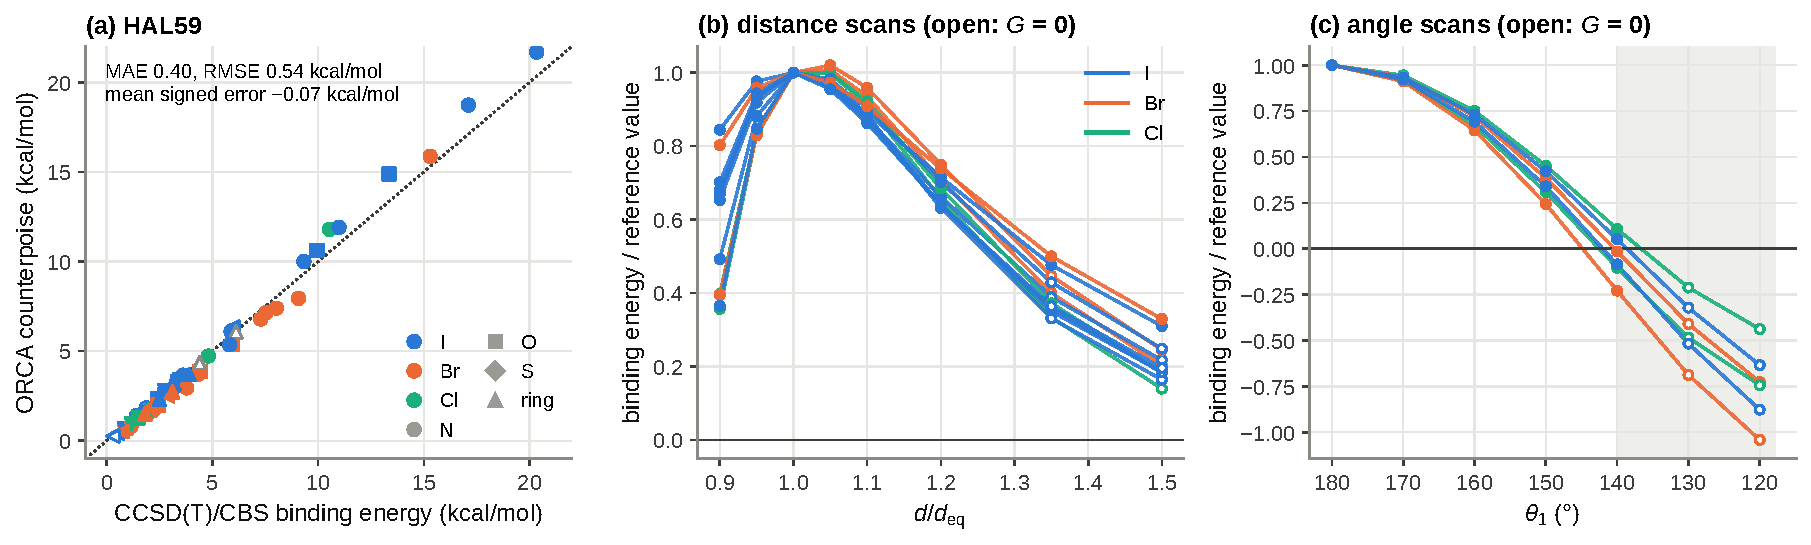
\includegraphics[width=\textwidth]{Fig6_CP_benchmark.pdf}
\caption{Counterpoise-corrected interaction energies from ORCA ($\omega$B97X-V/def2-TZVPD, gas phase). (a) Binding energies of the 59 HAL59 dimers against CCSD(T)/CBS (colour: halogen; shape: acceptor as in Figure~\ref{fig:t1}; open symbols: controls; dotted line: identity). (b) Binding energy along the 12 rigid distance scans relative to the value at $d_\mathrm{eq}$ (open symbols: $G = 0$). (c) Binding energy along the six rigid angle scans relative to the value at \ang{180} (shaded: outside the T1 angle window).}
\label{fig:cp}
\end{figure*}

Along the distance scans (Figure~\ref{fig:cp}b), 63--75\% of the binding energy remains at 1.20~$d_\mathrm{eq}$, 14--33\% at 1.50~$d_\mathrm{eq}$, and 36--88\% at the first point with $G = 0$, so the T1 cut-offs select close contacts rather than the whole attraction, while at 0.90~$d_\mathrm{eq}$ the binding energy falls to 36--84\% of its maximum although $G$ is unchanged or higher. Along the rigid angle scans (Figure~\ref{fig:cp}c), the binding energy falls monotonically, with 24--45\% of the linear value remaining at \ang{150}, between $-23$ and $+11$\% at \ang{140}, and repulsion for all six dimers at \ang{130}; because part of this repulsion is steric, the scans show that $\theta_1 \ge \ang{140}$ is conservative for rigid contacts rather than that the attraction ends there.

\subsection{NBO screen on the benchmark}
% Original wording retained for reference; revised wording follows.
% Of the 41 XBs covered by T1, 40 are supported and one, CH$_3$Br$\cdots$benzene (0.73~\kcal{}, binding energy 1.81~\kcal{}), is inconclusive (Figure~\ref{fig:nbo}a, ESI Table~\ref{S-tab:qmhal}); of the 15 XBs with P or F acceptors, 13 are supported and MeI$\cdots$FCCH (0.41~\kcal{}) and Br$_2\cdots$FCCH (0.48~\kcal{}), with binding energies of only 0.50 and 0.74~\kcal{}, are inconclusive. Altogether, 53 of 56 XBs are supported (1.12--72.2~\kcal{}), three are inconclusive, none is rejected, and the three controls are not supported (0.00, 0.00, and 0.05~\kcal{}). $\Sigma\ET$ ranks the covered XBs like the reference ($\rho = 0.93$ [0.83, 0.98], $n = 41$; over all 56, $\rho = 0.87$ [0.75, 0.94]), grows from Cl to Br to I for a fixed partner (1.18, 2.54, and 4.08~\kcal{} with acetone and 1.97, 4.65, and 7.48~\kcal{} with trimethylamine), and follows the NPA charge transfer and the ALMO-EDA CT energy closely ($\rho = 0.97$ for both). In FI$\cdots$pyridine, NBO describes the donor as I$^+$ and F$^-$, and the pyridine lone pair donates 72.2~\kcal{} into the vacant LP$^*$ of iodine. The Rydberg part, which is not counted, has a median share of 7\% and a maximum of 19\% at these geometries.
\tcb{For the 29 HAL59 dimers with C-bound Cl, Br, or I donors, valence $\Sigma E^{(2)}_{\mathrm{core}}$ correlates with CCSD(T)/CBS binding energies with Spearman $\rho=0.7269$ ($p=7.98\times10^{-6}$). Twenty-seven are labelled supported and two inconclusive. Only 23 of these 29 dimers also satisfy the present T1 acceptor and geometry scope; among those 23, 22 are supported and one is inconclusive. The 27 non-C-bound-donor dimers, including FI$\cdots$pyridine with $\Sigma E^{(2)}=72.2$~kcal~mol$^{-1}$, remain exploratory QM cases and are not part of the T1 benchmark performance. The three nominal negative controls fail T1 and therefore do not test NBO specificity. The four T1-passing rigid angle-scan geometries with repulsive counterpoise energies are nevertheless NBO-supported. Thus, within the current T1 window, the NBO value reports donor--acceptor orbital donation and does not alone distinguish an attractive interaction from a repulsive, sterically compressed, or otherwise unfavorable contact. The requested relaxed bent repulsive contacts, type-I X$\cdots$X contacts, C--X$\cdots$H--N contacts, and crystal-packing-enforced negative controls are not present in the repository and have not been tested.}



\begin{figure*}[t]
\centering
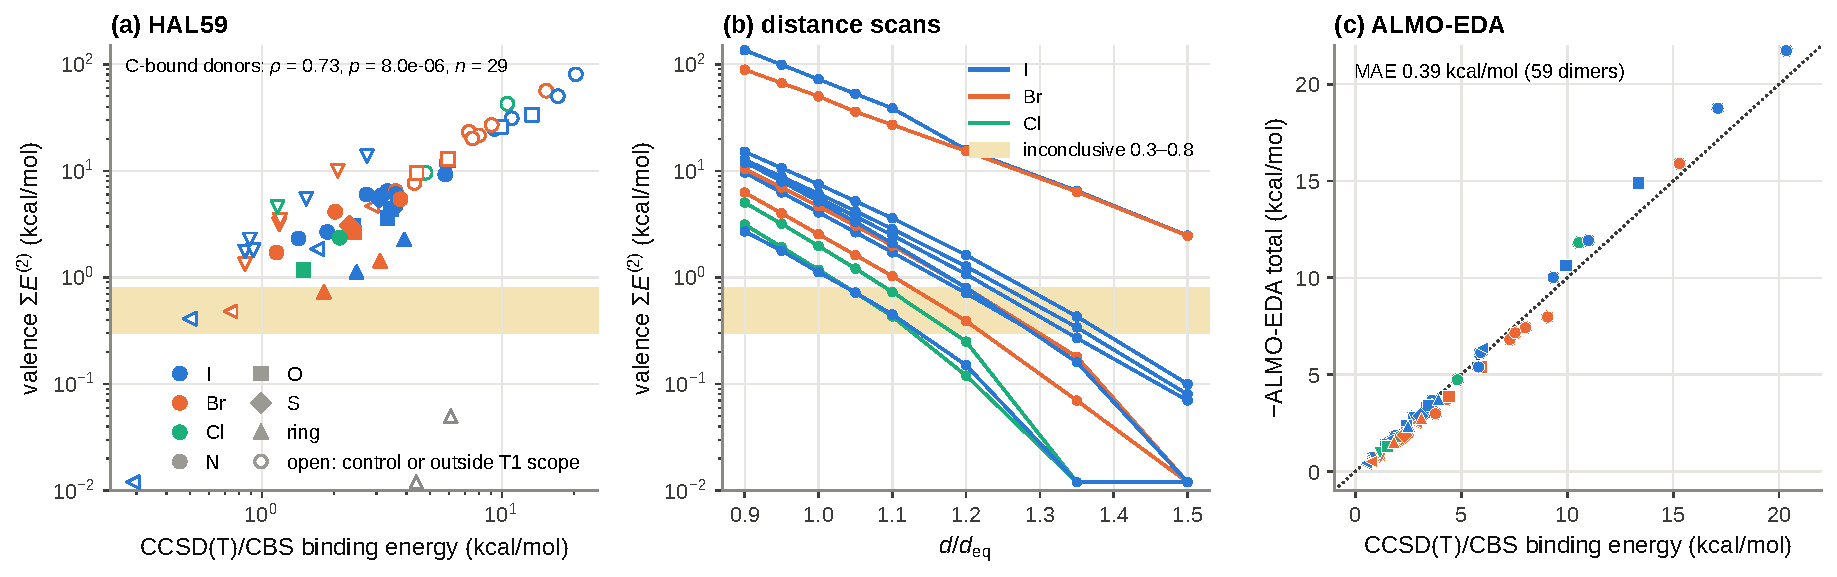
\includegraphics[width=\textwidth]{Fig7_NBO_benchmark.pdf}
\caption{NBO screen and ALMO-EDA on the HAL59 benchmark. (a) Valence $\Sigma\ET$ (Gaussian~16, $\omega$B97X-D/def2-TZVP) against the CCSD(T)/CBS binding energy (colour: halogen; shape: acceptor as in Figure~\ref{fig:t1}; open symbols: controls and P or F acceptors; zeros drawn at the lower axis limit; shaded: grey zone). (b) Valence $\Sigma\ET$ along the 12 distance scans (zeros drawn at 0.012~\kcal{}). (c) ALMO-EDA interaction energy ($\omega$B97X-V/def2-TZVPD) against the reference (dotted: identity).}
\label{fig:nbo}
\end{figure*}

% Original wording retained for reference; revised wording follows.
% $\Sigma\ET$ is not a binding energy, and its ratio to the binding energy depends on the acceptor class (ESI Table~\ref{S-tab:classratio} and Figure~\ref{S-fig:classes}a): the median ratio is 1.89 for N acceptors ($n = 26$), 1.18 for O acceptors ($n = 9$), and only 0.46 for the four ring acceptors, so the upper limit of 0.8~\kcal{} corresponds to about 0.4~\kcal{} of binding for an N acceptor, 0.7~\kcal{} for an O acceptor, and 1.8~\kcal{} for a ring. A single zone therefore under-scores ring acceptors about fourfold and O acceptors, which dominate protein contacts, by about one third relative to N acceptors, which explains why CH$_3$Br$\cdots$benzene is inconclusive while MeI$\cdots$NCH, with a smaller binding energy of 1.42~\kcal{}, is supported. With only four ring dimers, we do not fit a class-specific zone; instead, \BX{} flags ring contacts, and an inconclusive ring contact should be read as a possible weak halogen--$\pi$ bond.
\tcb{$\Sigma E^{(2)}$ is not a binding energy, and its ratio to the CCSD(T)/CBS binding energy depends on acceptor class (ESI Table~\ref{S-tab:classratio} and Figure~\ref{S-fig:classes}a). For the 29 C-bound-donor dimers, the median $E^{(2)}_{\mathrm{core}}/E_{\mathrm{bind}}$ ratios are 1.61 for N (n=12), 1.09 for O (n=5), 1.56 for S (n=2), 0.46 for ring acceptors (n=4), 2.01 for P (n=4), and 0.95 for F (n=2). P and F are outside the T1 acceptor scope. The O median is approximately 33\% lower than the N median, while the ring median is approximately 3.5-fold lower. These class differences show why a single NBO interval can under-score some acceptor classes, especially aromatic rings and O partners. We retain the common 0.3--0.8~kcal~mol$^{-1}$ interval as an operational screen and flag ring acceptors; no class-specific threshold has been calibrated against an independent energy criterion. With only four ring dimers in the C-bound subset, a separate ring threshold would be poorly determined.}

Along the distance scans (Figure~\ref{fig:nbo}b), $\Sigma\ET$ falls monotonically, keeping only 10--31\% of its equilibrium value at 1.20~$d_\mathrm{eq}$ (where the binding energy keeps 63--75\%), and at 1.50~$d_\mathrm{eq}$ ten contacts are not supported and two remain supported, so the screen selects close contacts with strong orbital overlap. At 0.90~$d_\mathrm{eq}$, however, $\Sigma\ET$ rises to 1.8--2.7 times its equilibrium value, and in the angle scans it keeps 52--57\% of its linear value at \ang{140} and 17--21\% at \ang{120}, where two contacts are still supported, three are inconclusive, and one is not supported, although the counterpoise energy is repulsive from \ang{130} on (ESI Figure~\ref{S-fig:angqm}). Of the 102 scan geometries that pass T1, four (all at \ang{140}) have a repulsive counterpoise energy, and the screen supports all four (ESI Figure~\ref{S-fig:gatecal}a). Measured against an energy criterion, the screen therefore has no specificity within the T1 window: it confirms that a lone pair donates into the $\sigma$-hole, not that the contact is attractive, so the geometric limits remain part of the decision and compressed contacts are flagged separately by $R < 0.80$.

\paragraph{Level of theory and the grey zone.}
% Original wording retained for reference; revised wording follows.
% Relative to $\omega$B97X-D/def2-TZVP, the level of theory changes the valence $\Sigma\ET$ of the 12 scan dimers by factors of 0.68 (chlorobenzene$\cdots$acetone with def2-SVP) to 1.17 (CH$_3$I$\cdots$benzene with def2-QZVP), whereas M06-2X, B3LYP-D3(BJ), and PBE0-D3(BJ) give 0.74--0.89 and Hartree--Fock 0.77--0.99; no decision changes, the smallest value at any level is 0.80~\kcal{}, and the ranking is preserved ($\rho \ge 0.98$; ESI Figure~\ref{S-fig:mb} and Table~\ref{S-tab:levels}). The Rydberg terms, in contrast, inflate the sum with Rydberg donation counted by up to a factor of 2.7 with def2-QZVP, which is why they are not counted. The protein model variants change the valence value of a contact by factors of 0.94 (Asn65 in the gas-phase cluster) to 1.27 (Thr113 in QM/MM with the Z3 scheme), and combining the two spreads (0.63--1.49) maps the conventional centre of 0.5~\kcal{} onto 0.34--0.79~\kcal{}. Because the protein maximum comes from the Thr113 contact, whose model carries the hydroxyl artefact discussed below, we repeated the derivation without it: the protein maximum becomes 1.16 (Phe80 with the Z1 scheme), the combined spread 0.63--1.36, and the zone 0.37--0.79~\kcal{}. We use the rounded and slightly wider zone of 0.3--0.8~\kcal{} in both cases (ESI Figure~\ref{S-fig:gatecal}b); a value inside it means that a plausible change of method or model could reverse the decision.
\tcb{Relative to $\omega$B97X-D/def2-TZVP, the level of theory changes valence $\Sigma E^{(2)}$ for the 12 scan dimers by factors of 0.68--1.17; M06-2X, B3LYP-D3(BJ), and PBE0-D3(BJ) give 0.74--0.89, and Hartree--Fock gives 0.77--0.99. No classifications change within this 12-dimer level test, the smallest value at any level is 0.80~kcal~mol$^{-1}$, and the ranking is preserved ($\rho\geq0.98$; ESI Figure~\ref{S-fig:mb} and Table~\ref{S-tab:levels}). The Rydberg terms can inflate the total donation and are therefore reported separately. Protein model variants change a contact by factors of 0.94--1.27 relative to its default model; combining the level and model spreads maps the selected 0.5~kcal~mol$^{-1}$ reference to approximately 0.34--0.79~kcal~mol$^{-1}$. The 0.5 value is an operational reference within the 0.3--0.8 interval, not its arithmetic midpoint or an energy-calibrated threshold. The 0.3--0.8 interval is retained as a deliberately inclusive screening region. The acceptor-class ratios above demonstrate that this single interval is not class-neutral; class-specific calibration remains outstanding.}

\subsection{Contacts with poor Lewis bases}
% Original wording retained for reference; revised wording follows.
\tcb{The three original HAL59 controls are easy negatives because they fail T1 before NBO is applied. The 18 halogen$\cdots$N, O, or S pairs inside the default protein clusters do not provide an independent NBO-negative set: six fail T1 and never reach the screen. The additional hIYD challenge set G supplies 12 T1-passing poor-Lewis-base contacts and five Lewis-base comparison contacts. Among the 12 poor-Lewis-base contacts, seven are not supported, three are inconclusive, and two are supported (Arg164 and Thr178). This challenge set shows that the poor-Lewis-base flag does not automatically determine the NBO verdict, but it is not a substitute for relaxed repulsive, type-I X$\cdots$X, C--X$\cdots$H--N, or crystal-packing hard negatives. Four T1-passing rigid angle-scan structures also have repulsive counterpoise energies while remaining NBO-supported; their rigid nature limits how strongly they can be generalized to relaxed structures.}

\subsection{Electronic tiers for the protein contacts}

\begin{figure*}[t]
\centering
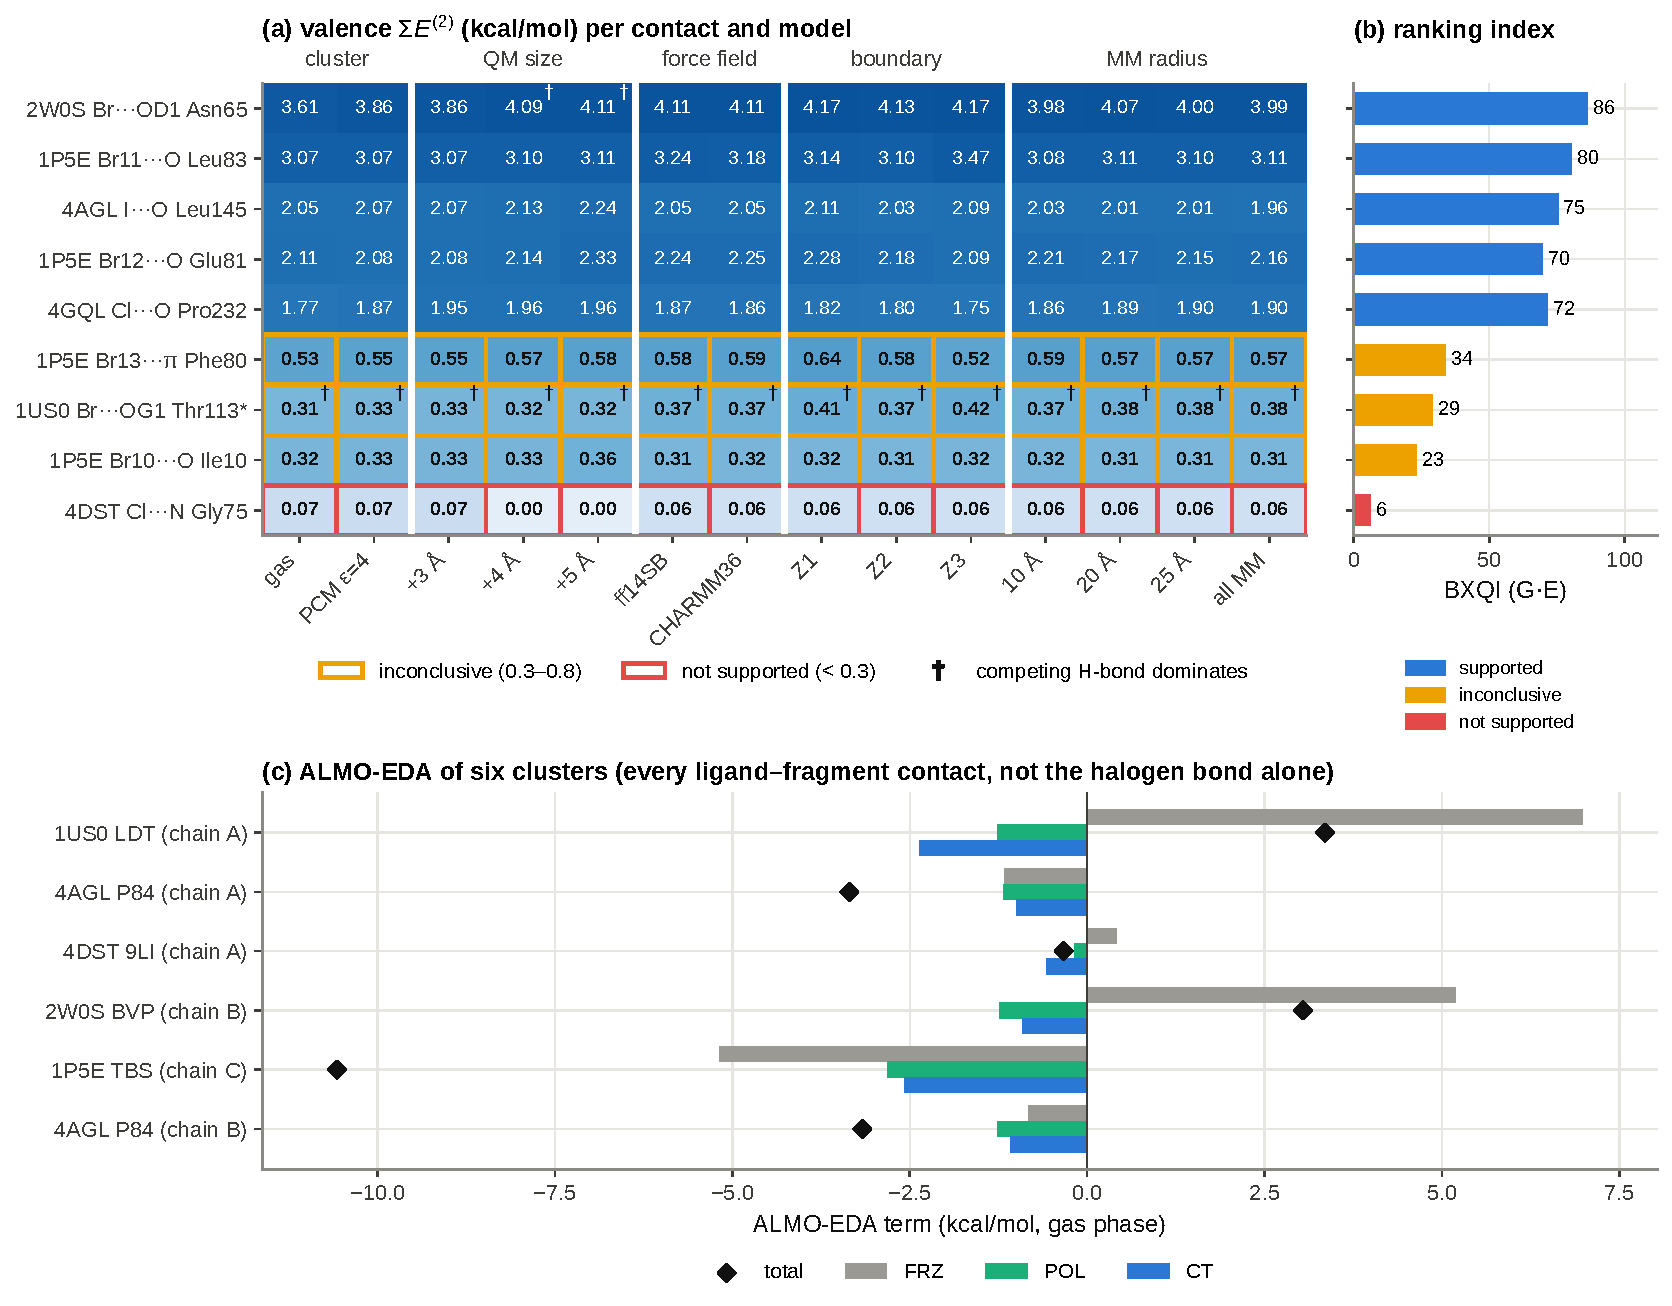
\includegraphics[width=\textwidth]{Fig8_protein_QM.pdf}
% Original wording retained for reference; revised wording follows.
% \caption{Electronic tiers for the protein contacts. (a) Valence $\Sigma\ET$ (Gaussian~16, $\omega$B97X-D/def2-TZVP) of nine contacts in 14 models; QM/MM models use ff14SB, the RC boundary, and \SI{15}{\angstrom} unless the column says otherwise, and the two His110 variants of 1US0 are listed in ESI Table~\ref{S-tab:qmprot}. Orange frames: inconclusive; red frames: not supported; $\dagger$: competing hydrogen bond dominates. All models were built with \BX{} with: a backbone N acceptor received a link hydrogen in place of the preceding carbonyl carbon (4DST Gly75), added hydroxyl hydrogens kept their template rotamer (1US0 Thr113), MM hydrogen charges were folded everywhere, and the QM/MM embedding radius was \SI{15}{\angstrom}. $^*$The 1US0 file also lacks NADP$^+$. (b) BXQI from $G$ and the default $\Sigma\ET$, coloured by the NBO decision. (c) ALMO-EDA terms of the six finished cluster jobs ($\omega$B97X-V/def2-TZVPD, gas phase; diamonds: total), which cover every contact between the ligand and the acceptor fragment, not the halogen bond alone.}
\caption{\tcb{Protein QM-model sensitivity. (a) Valence $\Sigma E^{(2)}$ across cluster size, force-field, boundary, and MM-radius variants. (b) BXQI ranking. (c) ALMO-EDA FRZ, POL, and CT terms for six ligand--environment cluster models; the horizontal scale is set from the full plotted range so positive FRZ contributions are not clipped. Protein models are described by their saved structural and embedding choices in the text; no application-edition distinction is implied.}}
\label{fig:prot}
\end{figure*}




Six of the nine ALMO-EDA jobs of the protein clusters finished (Figure~\ref{fig:prot}c, ESI Table~\ref{S-tab:proteda}); the jobs for 2W0S chain A, 1P5E chain A, and 4GQL stopped during the fragment calculations without a result, and the ORCA counterpoise job of 4GQL was not run. The finished totals agree with the ORCA counterpoise energies within 0.11~\kcal{}: the 1P5E cluster of chain C binds most strongly ($-10.57$~\kcal{}), whereas the 1US0 cluster and the 2W0S cluster of chain B are repulsive overall ($+3.35$ and $+3.04$~\kcal{}), because their anionic ligands face neutral acceptor fragments, although their CT terms are attractive ($-2.36$ and $-0.91$~\kcal{}). For the anionic 2W0S ligand, the Gaussian counterpoise energy with def2-TZVP (7.75~\kcal{}) differs strongly from the ORCA value with def2-TZVPD (3.07~\kcal{}), which shows that anions need diffuse functions. Because the cluster energies cover every ligand--fragment contact, BXQI for the protein contacts uses $G$ and $\Sigma\ET$ only (Figure~\ref{fig:prot}b): the supported contacts reach 51--86, the inconclusive ones 23--34, and the 4DST contact 6, and the ranking by decision keeps every supported contact above every inconclusive one.

\subsection{Case study: iodotyrosine release from hIYD}
Human iodotyrosine deiodinase releases its substrate I-Tyr along three pathways,\cite{Karmakar2026} and we applied tiers T0, T1, T2, T3b, and T5 to the published data of this release, reading the published QM models as they are and rebuilding only the backbone-N poses (set K). A fixed-charge force field gives the iodine one negative point charge, which repels a Lewis base from every direction and cannot produce a directional XB,\cite{Ibrahim2011,Rendine2011,KolarHobza2016} so the hIYD runs used an EP that mimics the $\sigma$-hole:\cite{Clark2007,Ibrahim2011,KolarHobza2012,Jorgensen2012} a positive charge \SI{2.15}{\angstrom} beyond the iodine on the C--I axis, held collinear by a stiff angle term and acting only through its charge (iodine $-0.278$~e, EP $+0.026$~e; ESI Table~\ref{S-tab:ep}). Control runs without the EP changed the release mechanism and removed most persistent contacts of the XB type,\cite{Karmakar2026} so a geometric screen of a trajectory reports the force field as much as the protein, and linear C--I$\cdots$Y contacts in an EP trajectory are only candidates for the electronic tiers.



\begin{figure*}[t]
\centering
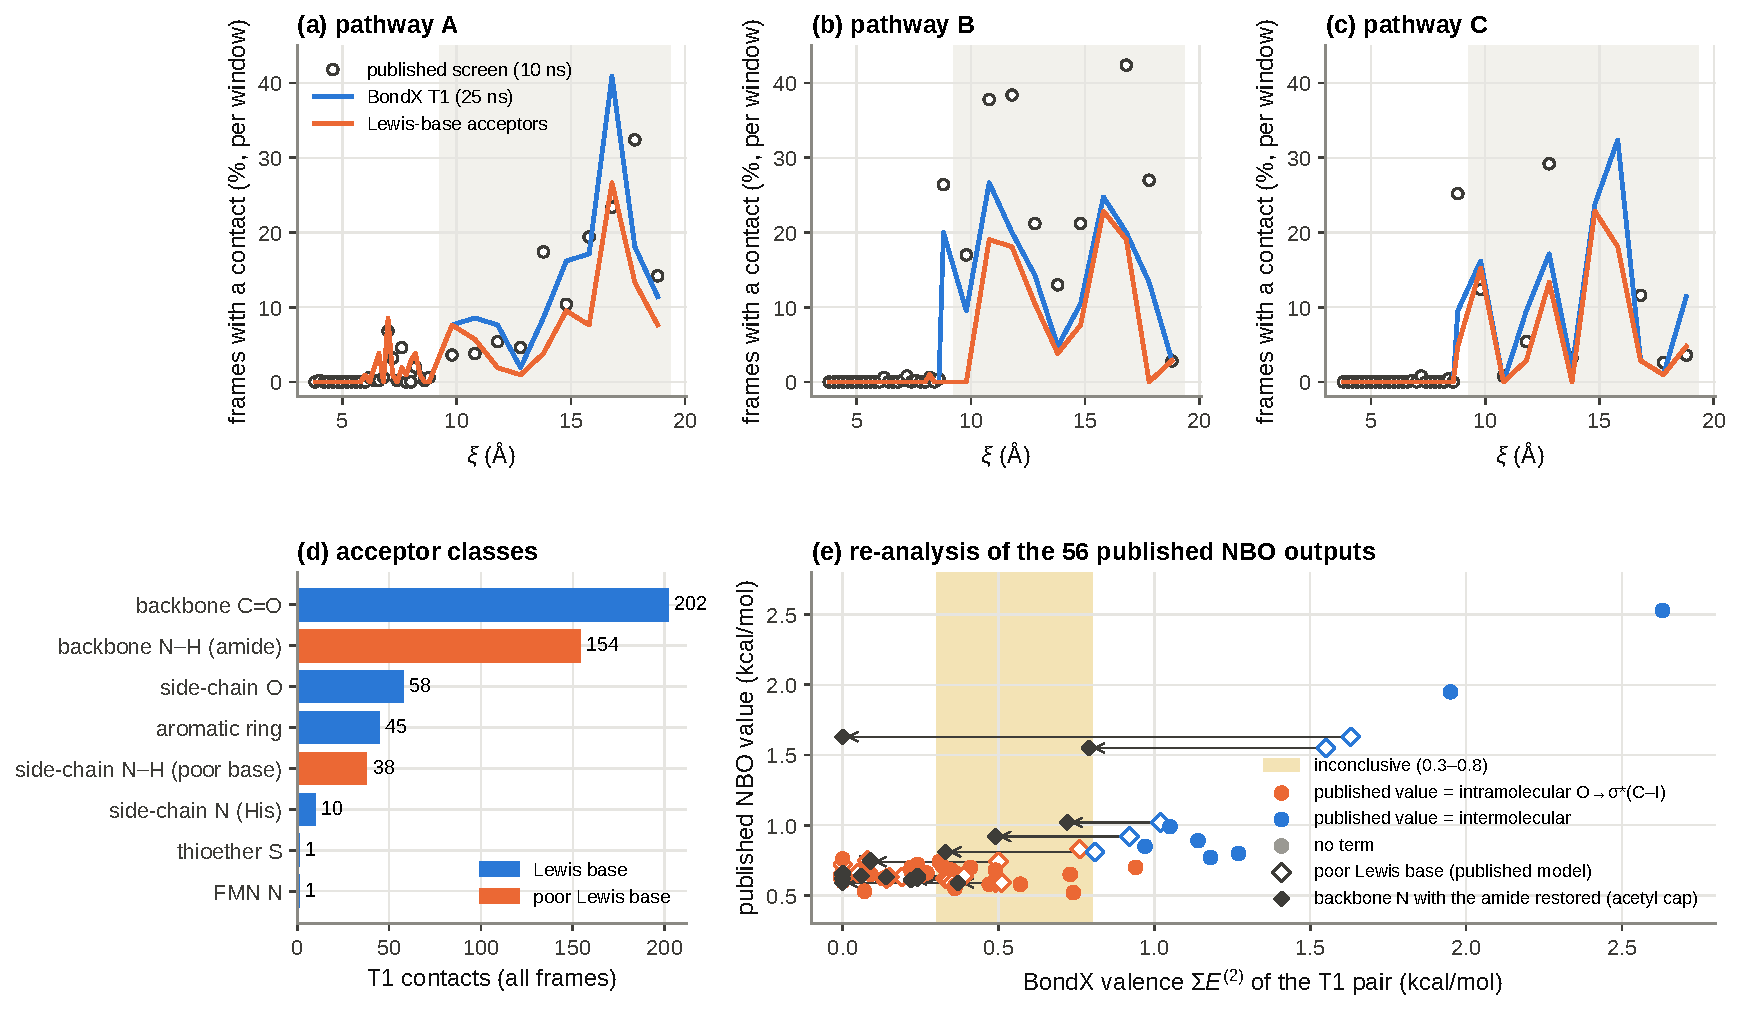
\includegraphics[width=\textwidth]{Fig9_hIYD.pdf}
\caption{\BX{} on the hIYD release of I-Tyr. (a--c) Share of frames with a T1 contact in each umbrella-sampling window of pathways A--C (unweighted, per window): published screen (open circles; first 10~ns, all acceptors including water), \BX{} T1 (blue; 25~ns), and \BX{} T1 with Lewis-base acceptors only (orange); windows are \SI{0.2}{\angstrom} apart below \SI{9}{\angstrom} and \SI{1}{\angstrom} apart in the shaded range. (d) Acceptor classes of the 509 T1 contacts (orange: poor Lewis bases). (e) Published NBO value against the \BX{} valence $\Sigma\ET$ of the T1 pair for the 56 published outputs (colour: origin of the published value; open diamonds: poor Lewis base in the published model; arrows and filled diamonds: backbone N with the amide restored by an acetyl cap; band: grey zone).}
\label{fig:hiyd}
\end{figure*}

\paragraph{Geometry and persistence.}
% Original wording retained for reference; revised wording follows.
% The first 10~ns of the published screen share 4793 frames with the stripped trajectories, and in these frames \BX{} found all 209 published contacts with protein or FMN atoms and no additional one, with distances and angles within the rounding of the published values; because both screens use the same criteria, this is a regression test of the implementation rather than an independent validation. Contacts are rare in the pocket ($\xi \le \SI{8.8}{\angstrom}$, 0.4--1.0\% of the frames of a window) and more frequent near the protein surface ($\xi \ge \SI{9.8}{\angstrom}$, 11.6--14.7\%, with a maximum of 41\% in pathway A at $\xi = \SI{16.8}{\angstrom}$; Figure~\ref{fig:hiyd}a--c). Of the 509 T1 contacts in all 11\,361 frames (Figure~\ref{fig:hiyd}d, ESI Table~\ref{S-tab:hiydclasses}), backbone carbonyl O atoms are the most frequent acceptors (202), followed by backbone amide N atoms (154), and the N--H groups of Arg, Lys, Asn, and Trp side chains add 38, so 192 contacts (38\%) involve poor Lewis bases that a pure distance-and-angle screen counts as XBs; with the Lewis-base filter, the share of frames with a contact for $\xi \ge \SI{9.8}{\angstrom}$ falls to 8.1--10.4\%. Tier T2, with the reporting threshold set to zero, gives 144 contacts in 42 windows (ESI Figure~\ref{S-fig:hiydt2}), with occupancies of at most 26\% (backbone O of L259 in pathway A at $\xi = \SI{16.8}{\angstrom}$), only ten above 10\%, and a highest pocket occupancy of 20\% (backbone N of A130$^*$). The saved frames of the windows with contacts are 160--240~ps apart, so 75\% of the contacts do not persist beyond one saved frame, the residence times (160--960~ps, median 240~ps) are resolved only to the frame spacing, and $D/f \ge 0.95$ makes $D$ practically equal to the occupancy (ESI Table~\ref{S-tab:hiydt5}); at this sampling, tier T2 contributes occupancies but no independent persistence information, and the program now says so.
\tcb{The first 10~ns of the published screen share 4,793 frames with the stripped trajectories, and in these frames the parser reproduces all 209 published contacts with protein or FMN atoms and no additional one; because the same geometric criteria are used, this is an implementation regression check rather than independent validation. Contacts are rare in the pocket ($\xi\leq8.8$~\AA{}, 0.4--1.0\% of a window) and more frequent near the protein surface ($\xi\geq9.8$~\AA{}, 11.6--14.7\%, with a maximum of 41\% in pathway A at $\xi=16.8$~\AA{}). Of 509 T1 contacts in 11,361 frames, backbone carbonyl O atoms are most frequent (202), followed by backbone amide N atoms (154); 192 contacts (38\%) involve poor Lewis bases. With the Lewis-base filter, the share of frames with a contact for $\xi\geq9.8$~\AA{} falls to 8.1--10.4\%. With the T2 reporting threshold set to zero, 144 contacts occur in 42 windows, with occupancies up to 26\%. Saved frames are 160--240~ps apart; for $\tau_0=100$~ps and $p=1/4$, $D/f$ is at least approximately 0.95, so D is practically the occupancy rather than an independent persistence discriminator. The umbrella-window occupancies are unweighted and window-specific, not unbiased ensemble populations. No finely sampled T2 trajectory test or WHAM/MBAR reweighting has been performed.}


\paragraph{NBO re-analysis.}
% Original wording retained for reference; revised wording follows.
% The published study tested one pose per residue by NBO,\cite{Karmakar2026} and \BX{} and an independent second parser read identical terms from all 56 outputs. The published value of each residue was the largest single LP(O, N, or S)$\to\sigma^*$(C--I) term of its output, which is not always an XB term: in 54 clusters, the phenolate O of I-Tyr, which sits ortho to the iodine, donates 0.52--0.83~\kcal{} into the $\sigma^*$(C--I) orbital of its own ring, and this intramolecular term was the published value in 43 clusters. All 18 published models with a backbone N acceptor contain the N with one heavy-atom neighbour and two hydrogens, that is, an amine instead of an amide. Counting only the T1 acceptor, the published models give 13 supported, 21 inconclusive, and 22 unsupported poses, but five of the supported poses are backbone-N amines (0.81--1.63~\kcal{}); once the amide is restored by an acetyl cap at the same pose and level (set K), none of the 18 backbone-N poses remains supported (five inconclusive at 0.33--0.79~\kcal{} and 13 not supported), and eight of them show N--H$\cdots$I hydrogen bonds that exceed the $\sigma$-hole donation (0.97--4.60~\kcal{}; Figure~\ref{fig:hiyd}e and ESI Table~\ref{S-tab:hiydnbo}). With these corrected models, the 56 poses give 8 supported, 19 inconclusive, and 29 unsupported contacts. Seven of the eight supported poses involve Lewis bases without a dominant competing hydrogen bond (N160 OD1, L259 O, Y211$^*$ OH in two pathways, K207$^*$ O, V209$^*$ O, and M165 SD; 0.94--2.63~\kcal{}), whereas the FMN N5 pose (1.95~\kcal{}) carries the flag, because its N5--H$\cdots$I hydrogen bond receives 5.65~\kcal{}. These outputs use a different level of theory from the one on which the grey zone was derived, so the class boundaries are approximate for them.
\tcb{The published study tested one pose per residue by NBO, and BondX Studio and an independent parser read identical terms from all 56 archived outputs. The published value for each residue was the largest single donor--acceptor term in the output; in 43 of 56 cases this was intramolecular donation from the phenolate O of I-Tyr into its own C--I antibond, rather than a protein--ligand XB term. All 18 published models with a backbone-N acceptor represented that nitrogen as an amine with one heavy-atom neighbour and two hydrogens, not as an intact amide. Counting only the T1 acceptor, the original models gave 13 supported, 21 inconclusive, and 22 unsupported poses. Rebuilding the 18 backbone-N poses with acetyl caps at the published level (set K) gave 13 not supported and five inconclusive; none was supported in that capped set. This result does not establish that intact amides are unsupported at every level of theory. In set G, the intact-amide Thr178 pose (pathway C, $\xi=15.8$~\AA{}; $d=3.53$~\AA{}; $\theta_1=178.1^\circ$) gives $\Sigma E^{(2)}=0.94$~kcal~mol$^{-1}$ and is supported at $\omega$B97X-D/def2-TZVP/CPCM ($\varepsilon=4$); the same geometry with an acetyl cap at the published level gives 0.79~kcal~mol$^{-1}$ and is inconclusive. Separately, all three set-J intact-amide 4DST Gly75 models give 0.00~kcal~mol$^{-1}$ and are not supported. The 56 hIYD poses with the rebuilt backbone-N models give eight supported, 19 inconclusive, and 29 unsupported contacts; these results use a different level from the grey-zone derivation and the classes should be interpreted accordingly.}


\paragraph{Consequences for our earlier study.}
% Original wording retained for reference; revised wording follows.
% This re-analysis affects the per-residue NBO statements of ref.~\citenum{Karmakar2026}. Its reported NBO values were the largest single donor--acceptor term of each output, which in 43 of 56 cases was the intramolecular phenolate donation, and its models of backbone-N acceptors, including the Thr178 and Ala130$^*$ poses used for the published basis-set tests, contained amines instead of amides; restoring the amides removes every supported backbone-N contact. The NBO-based assignment of individual residues as halogen-bond partners and the basis-set tests on these two poses are therefore superseded by ESI Table~\ref{S-tab:hiydnbo}, whereas the conclusions that rest on the MD and free-energy data, namely the release pathways, the barriers, and the effect of the EP model, do not depend on the NBO step and are unaffected. A correction to ref.~\citenum{Karmakar2026} that points to this re-analysis is submitted together with this article. The case also shows two requirements that \BX{} enforces: the screen counts only the T1 acceptor, and the QM model keeps the chemistry of the acceptor.
\tcb{This re-analysis affects the per-residue NBO statements of ref.~\citenum{Karmakar2026}. In 43 of 56 archived outputs, the reported largest NBO term was intramolecular phenolate donation. The published backbone-N models, including Thr178 and Ala130$^*$, represented amines rather than intact amides. The acetyl-capped set-K results revise the assignments at the published level, but the intact-amide Thr178 result in set G shows that the outcome depends on the structural model and level of theory; a blanket statement that no intact backbone-amide contact can be supported is not justified. The NBO-based assignment of individual residues as halogen-bond partners and the basis-set tests on the affected poses should therefore be reconsidered in light of ESI Table~\ref{S-tab:hiydnbo}. The MD release pathways, barriers, and conclusions based on the free-energy data do not depend on the NBO assignment and are unaffected. A correction to the earlier publication is not stated as submitted here because no submission receipt or confirmation is present in the supplied materials. The case reinforces two requirements: the screen must count only the selected T1 acceptor, and the QM model must preserve that acceptor's chemical identity.}


\subsection{Performance}
T1 runs in linear time (ESI Figure~\ref{S-fig:perf}): the 9212-atom structure 1P5E takes \SI{105}{ms}, a tiled structure with 73\,696 atoms takes \SI{0.78}{s}, the trajectory tier analyses 1039 frames per second for 1P5E, and QM model building takes \SIrange{46}{206}{ms}. The QM jobs dominate the total cost, since the 591 ORCA single points of sets A--C took 14.3~h of wall time on one 40-core node, the 24 ORCA protein single points 8.3~h, the Gaussian NBO jobs of sets A--F 71.9~h (42.6~h for the protein models), and the ALMO-EDA jobs 58.8~h (23.0~h for the six finished protein jobs); running the NBO screen first and the EDA only for supported contacts therefore saves most of the cost of tier T4.

\subsection{Limitations}

% Original wording retained for reference; revised wording follows.
% \BX{} writes inputs and reads outputs but runs no QM job, and its tested NBO route is Gaussian~16 with NBO~3.1, while ORCA was used only for counterpoise energies and Q-Chem only for ALMO-EDA, so the ORCA and Q-Chem NBO routes are locked as untested. The NBO screen tests orbital donation, not attraction: it does not detect bent contacts that are repulsive or compressed contacts that are losing binding, its grey zone was derived for one level of theory, it under-scores ring acceptors about fourfold and O acceptors by about one third relative to N acceptors, and it supported two of 13 contacts with poor Lewis bases, so the T1 flags remain part of every decision. The 89 protein models were built with \BX{} 2.0 and differ from the current defaults in four respects (backbone-N link hydrogens, template hydroxyl rotamers, folded MM hydrogen charges, and a \SI{15}{\angstrom} embedding radius); the current defaults have QM results for 20 models (sets G and J), but not for 1US0 with oriented hydroxyl hydrogens or for a QM/MM model with explicit MM hydrogens and whole-structure embedding, and the marginal protein contacts were not recomputed at other levels. Ligand protonation uses a Kekul\'e structure and group rules, so basic amines, tetrazoles, and acyl sulfonamides are flagged but not assigned automatically, and a MOL2 file with a state from a pKa tool is the recommended route, as is a PROPKA state for His. The MM region has no polarization, no solvent, and no neutralization, QM--MM van der Waals terms are absent, periodic treatment covers orthorhombic boxes only, XTC and NetCDF trajectories need conversion, P and F acceptors have no default cut-offs, occupancies from biased simulations are unweighted, and $D$ carries no information beyond the occupancy when the frame spacing reaches $\tau_0$. Finally, the BXQI weights and saturation constants are conventions, and we do not report a correlation of BXQI with the benchmark binding energies, because its EDA term is itself a DFT binding energy.
\tcb{BondX Studio writes QM inputs and reads outputs but does not run the quantum-chemical jobs itself. The tested NBO route is Gaussian~16 with NBO~3.1; ORCA NBO and Q-Chem NBO routes remain unvalidated. The NBO screen measures orbital donation, not attraction: the three original HAL59 controls fail T1 before the NBO step, and four T1-passing rigid angle-scan geometries with repulsive counterpoise energies are nevertheless NBO-supported. Independent relaxed bent repulsive contacts, type-I X$\cdots$X contacts, C--X$\cdots$H--N contacts, and crystal-packing-enforced negatives remain to be tested. The 0.3--0.8~kcal~mol$^{-1}$ interval is operational, and class-specific energy-calibrated thresholds have not been established. The distance cut-offs are empirical screening values inherited from the hIYD analysis, not direct sums of Bondi radii. Hybridization-dependent $\theta_2$ targets for sp, sp$^2$, and sp$^3$ acceptors are implemented and covered by regression tests, but the hybridization assignment is heuristic and further chemical validation is warranted. The 89 set-F protein models used the saved settings described above: backbone-N boundary link hydrogens where the preceding carbonyl was omitted, template hydroxyl rotamers, folded MM hydrogen charges throughout, and a 15~\AA{} embedding radius. The alternative 1US0 hydroxyl rotamer, full explicit-MM-H whole-structure QM/MM NBO model, and marginal-contact calculations at additional levels have not been completed. Protein NBO calculations for anionic ligands in 1US0, 2W0S, and 4GQL used def2-TZVP without diffuse functions; def2-TZVPD NBO sensitivity calculations for these systems remain outstanding. The MM region is non-neutral and non-polarizable, with no explicit solvent; no counterion or charge-scaling sensitivity tests have been performed. Ligand protonation remains connectivity-based unless a pKa-derived MOL2/PQR state is supplied; basic amines, tetrazoles, and acyl sulfonamides are flagged rather than assigned unambiguously. Periodic treatment is limited to orthorhombic boxes, and XTC/NetCDF trajectories require conversion. Umbrella-window occupancies are unweighted; with 160--240~ps saved-frame spacing, T2 is practically equal to occupancy and provides no independently resolved persistence information. Finally, BXQI weights and saturation constants remain conventions, and BXQI has not been validated as a binding-free-energy predictor.}

%% =====================================================================
\section{Conclusions}
% Original wording retained for reference; revised wording follows.
% A short halogen contact is a hypothesis, and \BX{} makes testing it by quantum chemistry a routine step: the program builds QM cluster and QM/MM models with established force-field protonation states and charges, keeps exact bookkeeping between the structure and the QM output, shows every assumption, and records every choice. All generated inputs and returned outputs matched their manifests, the force-field charges reproduce the PDB2PQR references for every heavy atom and hydrogen tested, and the geometric tier recovered all literature-validated contacts of the protein test set. The valence NBO screen supported 53 of 56 benchmark XBs, left three weak ones inconclusive, supported none of the controls, and was stable across levels of theory and model variants; at the same time, it confirms donation into the $\sigma$-hole rather than attraction, it under-scores ring acceptors, and it supported two of 13 contacts with poor Lewis bases, so the geometric limits and the acceptor flags remain part of every decision. In proteins, five of nine distinct contacts were supported, three remained inconclusive, and the amide-N contact of 4DST was not supported, while the competing-hydrogen-bond flag exposed hydrogen bonds to the halogen in 1US0 and 2W0S. The hIYD re-analysis showed that an acceptor-specific screen and an intact acceptor chemistry are essential, since restoring the backbone amides removed every supported backbone-N contact and corrected our own earlier NBO assignments. \BX{} is free and runs in any browser, and we hope that it makes the electronic check a standard part of halogen-bond studies.
\tcb{BondX Studio provides a browser-based, traceable workflow for detecting geometric halogen contacts and preparing force-field-consistent QM-cluster and electrostatically embedded QM/MM inputs. It preserves atom mapping between the original structure and quantum-chemical output, records model assumptions, and reports NBO and ALMO-EDA analyses without running the QM calculations itself. The repository engine suite passes 123 automated tests, and the independent force-field reference comparisons pass. In HAL59, the 29 C-bound Cl/Br/I donor dimers give a Spearman correlation of $\rho=0.7269$ ($p=7.98\times10^{-6}$) between valence $\Sigma E^{(2)}_{\mathrm{core}}$ and CCSD(T)/CBS binding energies; 27 are labelled supported and two inconclusive. Only 23 of these dimers satisfy the current T1 acceptor scope, among which 22 are supported and one is inconclusive. The 27 non-C-bound-donor dimers are exploratory electronic-structure cases and are excluded from T1 performance claims. The three nominal controls fail T1 before NBO is applied, while four T1-passing rigid angle-scan geometries with repulsive counterpoise energies are nevertheless NBO-supported. The NBO screen therefore identifies orbital donation, not net attraction, and must be interpreted together with geometry, acceptor identity, and independent energetic evidence. Of nine distinct selected protein contacts, five are supported, three inconclusive, and one not supported; of four selected literature-annotated C--X contacts, Ile10 remains inconclusive. In hIYD, 43 of 56 published NBO values are intramolecular phenolate donation. Acetyl-capped backbone-N calculations at the published level give 13 unsupported and five inconclusive results, while intact-amide Thr178 is supported at a separate default level, demonstrating model and level dependence. Hybridization-dependent $\theta_2$ scoring is implemented for sp, sp$^2$, and sp$^3$ acceptors. Outstanding limitations include independent relaxed hard-negative families, class-calibrated NBO thresholds, diffuse-basis NBO tests for anionic protein ligands, MM-charge neutralization sensitivity, unbiased umbrella-window reweighting, and full explicit-hydrogen whole-structure QM/MM validation. BondX Studio is a screening and model-construction tool, not a predictor of binding free energies.}


%% =====================================================================
% \section*{Data and Software Availability}
% % Original wording retained for reference; revised wording follows.
% \BX{} runs online at \url{https://compchemsk.github.io/BondX-Studio/}. The repository \url{https://github.com/compchemsk/BondX-Studio} holds the single-file application, the source code, the 120 tests, and the tutorial under the MIT license, together with the paper scripts (also collected in one Jupyter notebook), the data sets, the parsed QM results, and all QM input files. The benchmark geometries come from GMTKN55, and the protein files come from the PLIP test suite and the PDB.


% \section*{Supporting Information}
% ESI (PDF): literature counts; assumptions of every tier; equations, parameters, and distance cut-offs; force-field validation including hydrogens; geometric tier; protein QM models and MM field tests; NBO screen, acceptor classes, grey-zone derivation, contacts with poor Lewis bases, and ALMO-EDA results; ORCA counterpoise energies; hIYD case study with T2; scripts and reproducibility; user guide.

\section*{Data and Software Availability}

\tcb{BondX Studio is freely accessible at \url{https://compchemsk.github.io/BondX-Studio/}. The source code and associated data are available at \url{https://github.com/compchemsk/BondX-Studio}.}

\section*{Supporting Information}

\tcb{The Supporting Information (ESI) includes literature counts, methodological assumptions, equations and parameters, force-field data, geometric screening results, QM/QM-MM models, NBO and ALMO-EDA analyses, counterpoise energies, the hIYD case study, computational scripts, reproducibility details, and a user guide.}

\section*{Author information}
\noindent\textbf{Corresponding Authors}

\noindent\textbf{Sabyashachi Mishra}$-$Department of Chemistry, Indian Institute of Technology, Kharagpur$-$721302, India; \url{https://orcid.org/0000-0002-2551-1021}; Email: mishra@chem.iitkgp.ac.in

%\noindent\textbf{Author}

\noindent\textbf{Soumyajit Karmakar}$-$Department of Chemistry, Indian Institute of Technology, Kharagpur$-$721302, India; \url{https://orcid.org/0000-0003-4867-0970}

\noindent\textbf{Author contributions}\\
The manuscript was written with contributions from all authors, and all authors have given their approval to the final version. Conceptualization, methodology, and computational analysis: S. Karmakar and S. Mishra; writing, original draft: S. Karmakar; writing (review and editing): S. Mishra.

\section*{Declaration of competing interest}
The authors declare that they have no conflicts of interest in the contents of this article.

\section*{Acknowledgements}
% Original wording retained for reference; revised wording follows.
% SK acknowledges the Prime Minister's Research Fellowship, the Ministry of Education, Government of India, Associate Membership of the Royal Society of Chemistry, Membership of the American Chemical Society, and IIT Kharagpur for support. SM acknowledges the support from SERB, DST, Govt. of India (CRG/2022/004088 and SR/FST/CSII-026/2013). This work used the resources of the Paramshakti supercomputing facility of IIT Kharagpur, established under the National Supercomputing Mission of the Government of India and supported by CDAC, Pune.
\tcb{SK acknowledges the Prime Minister's Research Fellowship, the Ministry of Education, Government of India, and IIT Kharagpur for support. SM acknowledges support from SERB, DST, Government of India (CRG/2022/004088 and SR/FST/CSII-026/2013). This work used the resources of the Paramshakti supercomputing facility of IIT Kharagpur, established under the National Supercomputing Mission of the Government of India and supported by CDAC, Pune.}


\begin{small}
\bibliography{References_V3}
\end{small}

\begin{tocentry}
\begin{center}
\includegraphics[width=0.96\textwidth]{TOC_graphic.pdf}
\end{center}
\end{tocentry}

% Outstanding before submission (not represented as completed): obtain diffuse-basis NBO results for 1US0, 2W0S, and 4GQL; run controlled MM charge-neutralization/charge-scaling tests; calculate the alternative 1US0 hydroxyl rotamer and explicit-MM-H whole-structure QM/MM model; add relaxed/type-I/H-bonded/crystal-packing hard negatives; perform acceptor-class threshold calibration and unbiased WHAM/MBAR reweighting; archive the source snapshot at Zenodo and insert its registered DOI; verify the status of any correction to ref. 20.
\end{document}
